\chapter{Of File Systems and Storage Models}
\label{chap:file systems}

\begin{quote}
{\em Disks are always full. It is futile to try to get more disk
space. Data expands to fill any void.} --
Parkinson's Law as applied to disks
\end{quote}

% XXX better graphic
\begin{figure}[hb]
	\raggedleft
	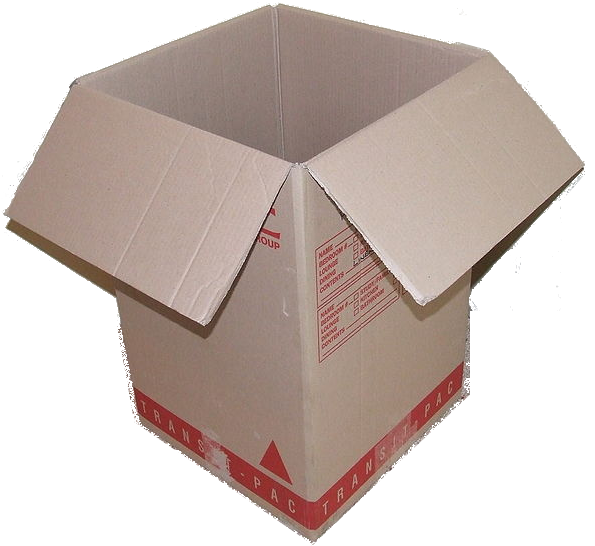
\includegraphics[width=.15\textwidth]{04/pics/box}
% XXX: no caption but label?
	\label{fig:storage-box}
\end{figure}


\section{Introduction}
\label{file systems:introduction}
\index{Storage Models}

This chapter deals primarily with how we store data.
Virtually all computer systems require some way to
store data permanently; even so-called ``diskless''
systems do require access to certain files in order to
boot, run and be useful.  Albeit stored remotely (or
in memory), these bits reside on some sort of storage
system.

Most frequently, data is stored on local hard disks,
but over the last few years more and more of our files
have moved ``into the cloud'', where different
providers offer easy access to large amounts of
storage over the network.  We have more and more
computers depending on access to remote systems,
shifting our traditional view of what constitutes a
storage device.

As system administrators, we are responsible for all
kinds of devices: we build systems running entirely
without local storage just as we maintain the massive
enterprise storage arrays that enable decentralized
data replication and archival.  We manage large
numbers of computers with their own hard drives, using
a variety of technologies to maximize throughput
before the data even gets onto a network.

In order to be able to optimize our systems on this
level, it is important for us to understand the
principal concepts of how data is stored, the
different {\em storage models} and {\em disk
interfaces}.  It is important to be aware of certain
physical properties of our storage media, and the
impact they, as well as certain historic limitations,
have on how we utilize disks.

Available storage space is, despite rapidly falling
prices for traditional hard disk drives, a scarce
resource\footnote{We will take a closer look a the
{\em Total Cost of Ownership\index{Total Cost of
Ownership}} of a hard drive in Chapter
\ref{chap:backup}.  Suffice it to say that the
purchase price of the storage device itself is only a
fraction.}.  The quote a the beginning of this chapter
is rather apt: no matter how much disk space we make
available to our users, we will eventually run out and
need to expand.  In order to accommodate the
ever-growing need for storage space, we use
technologies such as Logical Volume
Management\index{Logical Volume Manager} to combine
multiple physical devices in a flexible manner to
present a single storage container to the operating
system.  We use techniques such as
\glslink{raid}{RAID}\index{RAID} to increase capacity,
resilience or performance (pick two!), and separate
data from one another within one storage device using
partitions.  Finally, before we can actually use the
disk devices to install an operating system or any
other software, we create a file system on top of
these partitions.

System administrators are expected to understand well
all of these topics.  Obviously, each one can (and
does) easily fill many books; in this chapter, we will
review the most important concepts underlying the
different technologies from the bottom up to the file
system level.  At each point, we will compare and
contrast traditional systems with recent developments,
illustrating how the principles, even if applied
differently, remain the same.  For significantly
deeper discussions and many more details, please see
the chapter references, in particular the chapters on
file systems in
Silberschatz\cite{filesystems:silberschatz}\index[names]{Silberschatz,
Abram} and McKusick\index[names]{McKusick, Marshall
Kirk} et al.'s canonical paper on the Berkeley Fast
File System\cite{filesystems:ffs}.


\section{Storage Models}
\label{file systems:storage-models}

We distinguish different storage models by how the
device in charge of keeping the bits in place
interacts with the higher layers: by where raw block
device access is made available, by where a file
system is created to make available the disk space as
a useful unit, by which means and protocols the
operating system accesses the file system.  Somewhat
simplified, we identify as the main three components
the storage device itself, i.e. the actual medium; the
file system, providing access to the block level
storage media to the operating system; and finally the
application software.  The operating system managing
the file system and running the application software
then acts as the agent making actual I/O possible.

\subsection{Direct Attached Storage}
\label{file systems:storage-models:das}
\index{Direct Attached Storage}

The by far most common way to access storage is so
simple that we rarely think about it as a storage {\em
model}:  hard drives are attached (commonly via a host
bus adapter\index{Host Bus Adapter} and a few cables)
directly to the server, the operating system detects
the block devices and maintains a file system on them
and thus allows for access with the smallest level of
indirection.  The vast majority of hosts (laptops,
desktop and server systems alike) all utilize this
method.  The term used nowadays -- {\em \gls{das}
\index{Direct Attached Storage}} -- was effectively
created only after other approaches become popular
enough to require a simple differentiating name.

\begin{figure}[ht]
	\centering
	\subfloat[Diagram]{\label{fig:storage:das-diagram}
			\makebox[.35\textwidth]{
				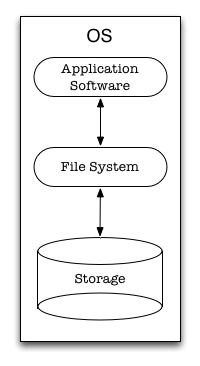
\includegraphics[width=.25\textwidth]{04/pics/das}}}
	\hspace{5em}
	\subfloat[A Maxtor IDE Drive]{\label{fig:storage:das-maxtor}
				\raisebox{2em}{
					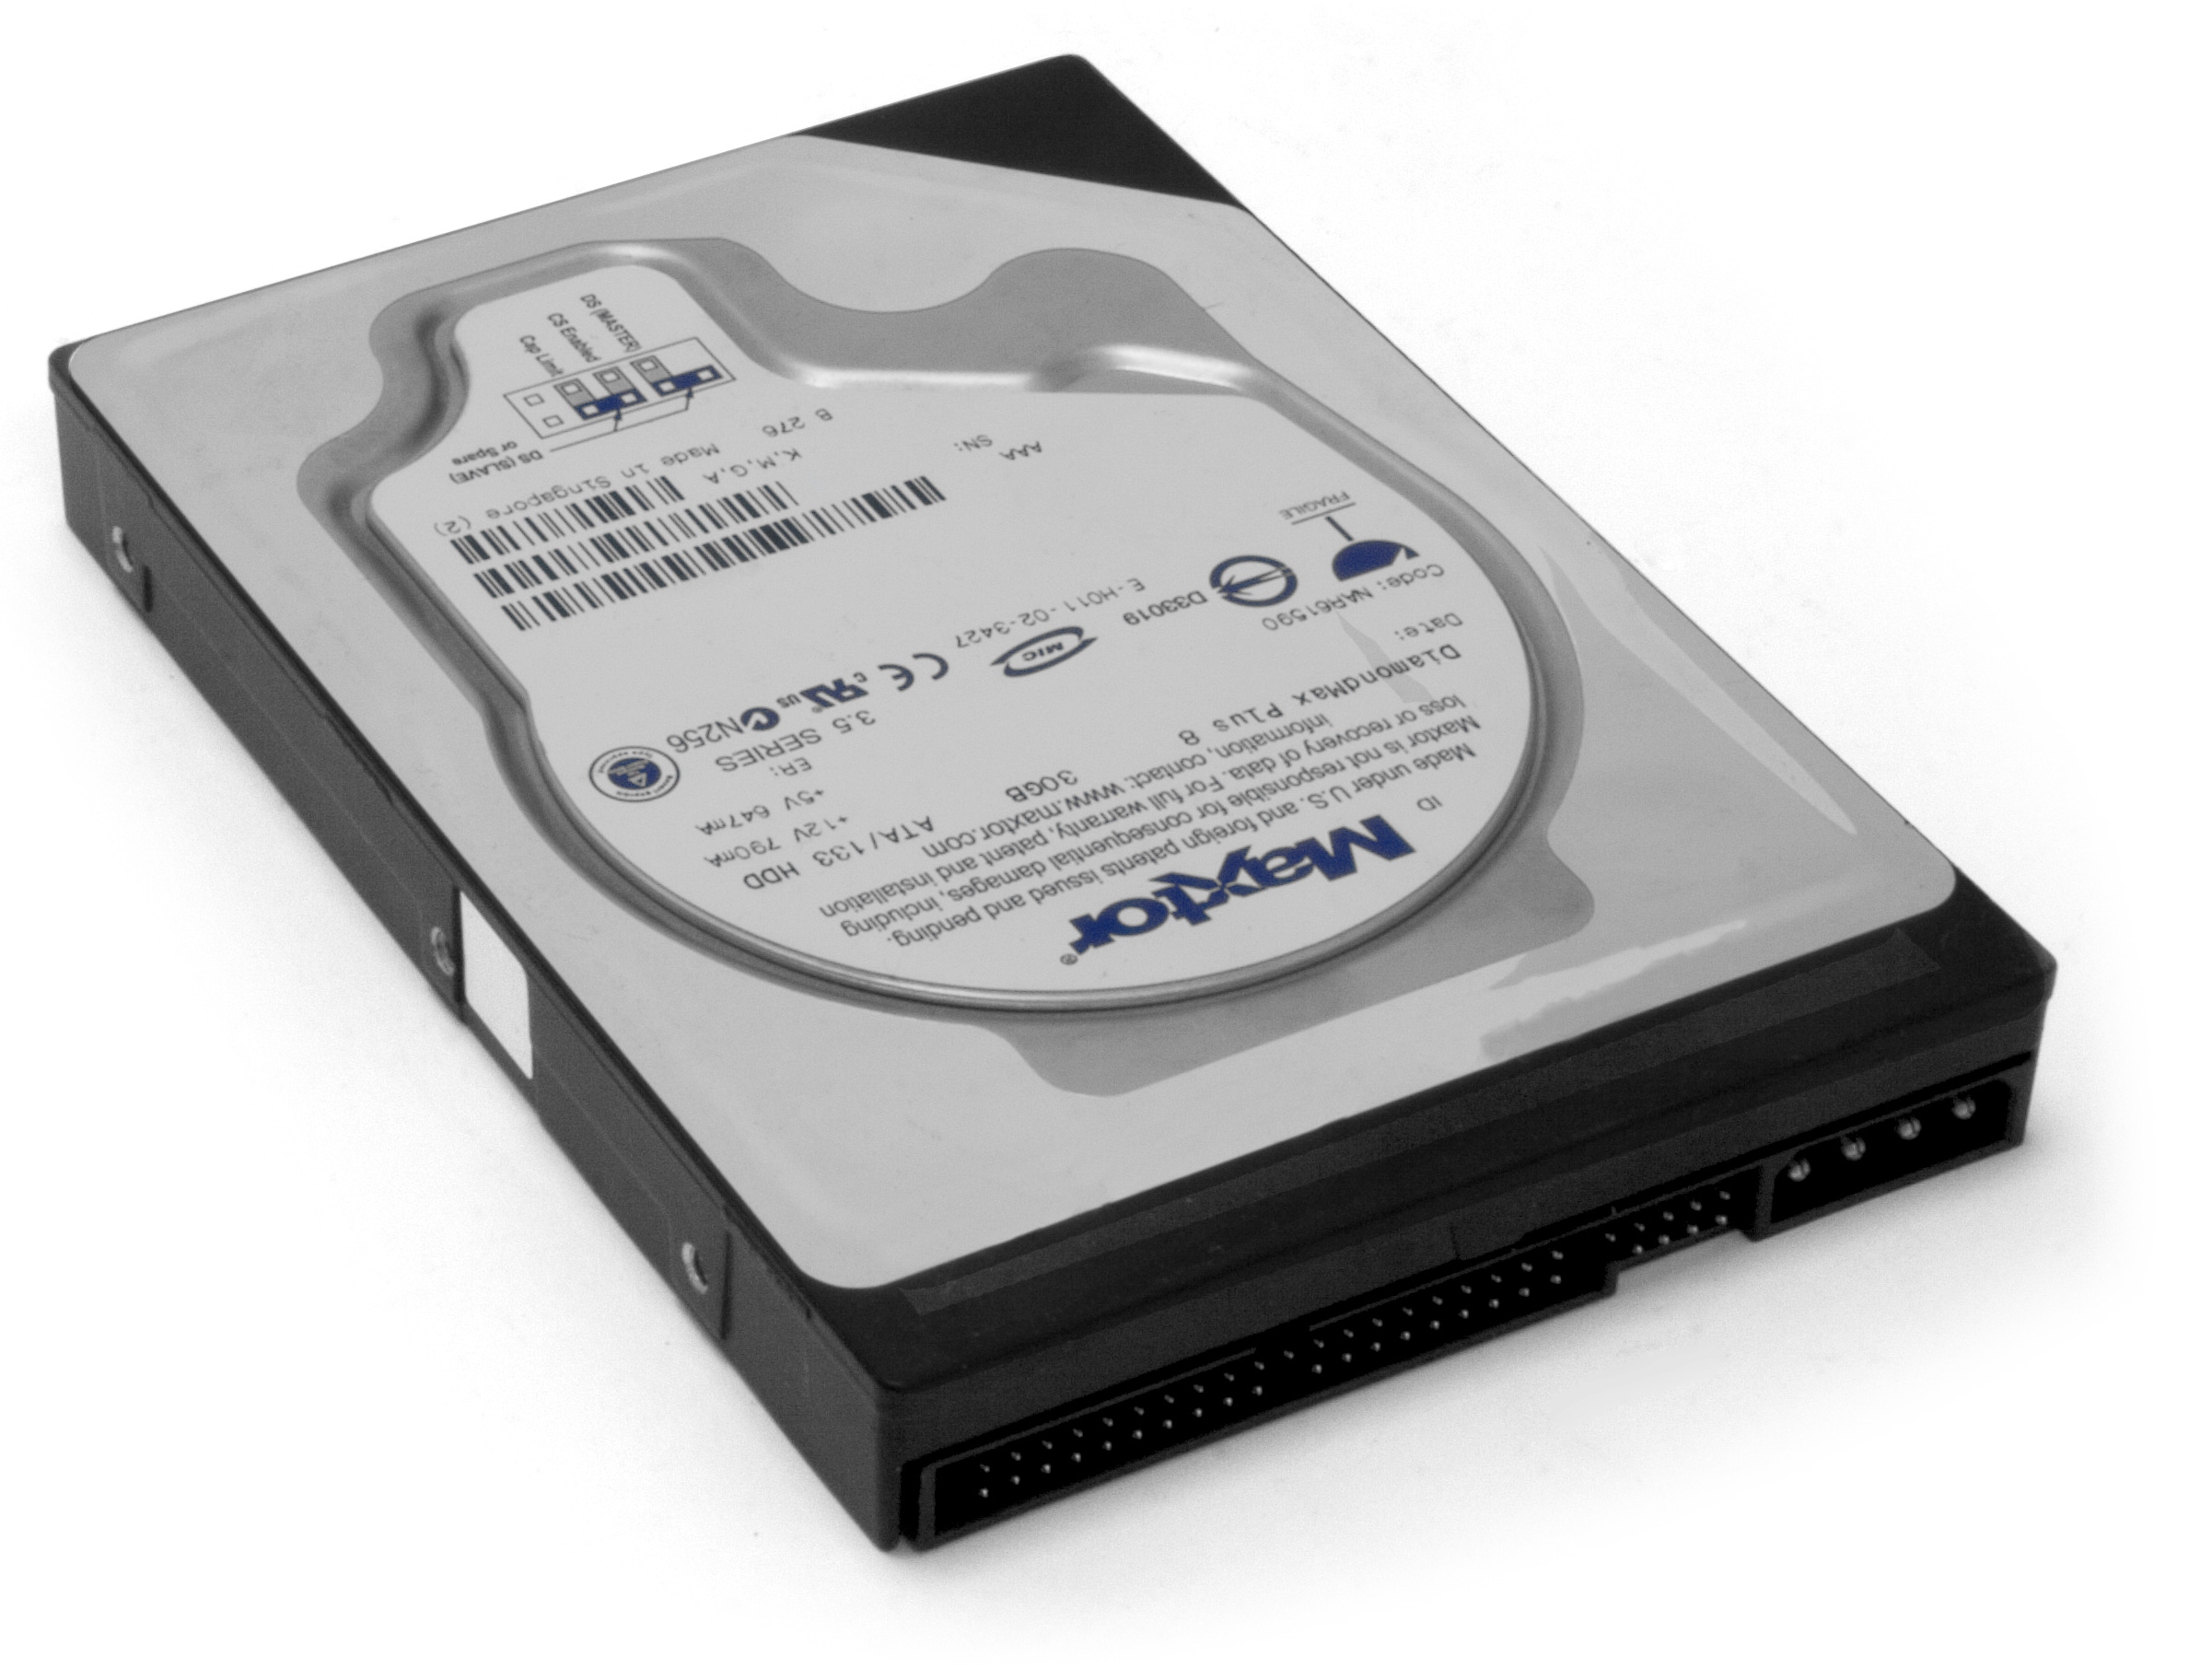
\includegraphics[width=.4\textwidth]{04/pics/maxtor}}}
	\caption{Direct Attached Storage}
\end{figure}


Figure \ref{fig:storage:das-diagram} illustrates this
model: all interfacing components are within the
control of a single server's operating system (and
frequently located within the same physical case) and
multiple servers each have their own storage system.
On the hardware level, the storage media may be
attached using a variety of technologies, and we have
seen a number of confusing standards come and go over
the years.  The best choice here depends on many
factors, including the number of devices to be
attached, driver support for the connecting interface
in the OS, and performance or reliability
considerations.  We will touch upon all of these
aspects throughout this chapter.

A server with a single hard drive (such as the one
shown in Figure \ref{fig:storage:das-maxtor} is
perhaps the simplest application of this model.  But
it is not uncommon for servers to have multiple direct
attached devices, the configuration of which then
depends entirely on the next higher level of storage
strategies.  Individual disks can simply be mounted in
different locations of the file system hierarchy.
Alternatively, multiple direct attached disks can be
combined to create a single logical storage unit
through the use of a \gls{lvm}\index{Logical Volume
Manager} or a \gls{raid}\index{RAID}.  This allows for
improved performance, increased amount of storage
and/or redundancy.  We will discuss these concepts in
more detail in Section \ref{file
systems:storage-models:dividing-and-combining-disks}.

Direct attached storage need not be physically located
in the same case (or even rack) as the server using
it.  That is, we differentiate between {\em internal}
storage (media attached inside the server with no
immediate external exposure) and {\em external}
storage (media attached to a server's interface ports,
such as Fibre Channel\index{Fibre Channel},
USB\index{USB} etc.) with cables the lengths of which
depend on the technology used.  External media allows
us to have large amounts of storage housed in a
separate enclosure with its own power supply, possibly
located several feet away from the server.  If a
server using these disks suffers a hardware failure,
it becomes significantly easier to move the data to
another host: all you need to do is connect the cable
to the new server.

Simple as this architecture is, it is also ubiquitous.
The advantages of \gls{das} should be obvious: since there
is no network or other additional layer in between the
operating system and the hardware, the possibility of
failure on that level is eliminated.  Likewise, a
performance penalty due to network latency, for
example, is impossible.  As system administrators, we
frequently need to carefully eliminate possible causes
of failures, so the fewer layers of indirection we
have between the operating system issuing I/O
operations and the bits actually ending up on a
storage medium, the better.

At the same time, there are some disadvantages.  Since
the storage media is, well, {\em directly} attached,
it implies a certain isolation from other systems on
the network.  This is both an advantage as well as a
drawback: on the one hand, each server requires
certain data to be private or unique to its operating
system; on the other hand, data on one machine
cannot immediately be made available to other systems.
This restriction is overcome with either one of the
two storage models we will review next: {\em \gls{nas}}\index{Network Attached Storage}
and {\em Storage Area Networks}\index{Storage
Area Network} (\glslink{san}{SAN}s).

\gls{das} can easily become a shared resource by
letting the operating system make available a local
storage device over the network.  In fact, all network
file servers and appliances ultimately are managing
direct attached storage on behalf of their clients;
DAS becomes a building block of {\em NAS}.  Likewise,
physically separate storage enclosures can function as
DAS if connected directly to a server or may be
combined with others and connected to network or
storage fabric, that is: they become part of a {\em
SAN}.\footnote{Don't worry, the various acronyms seem
confusing as they are introduced, but hardly anybody
actually utters sentences containing more than one.
One feels too silly doing so.}


\subsection{Network Attached Storage}
\label{file systems:storage-models:nas}
\index{Network Attached Storage}

\begin{figure}[ht]
	\centering
	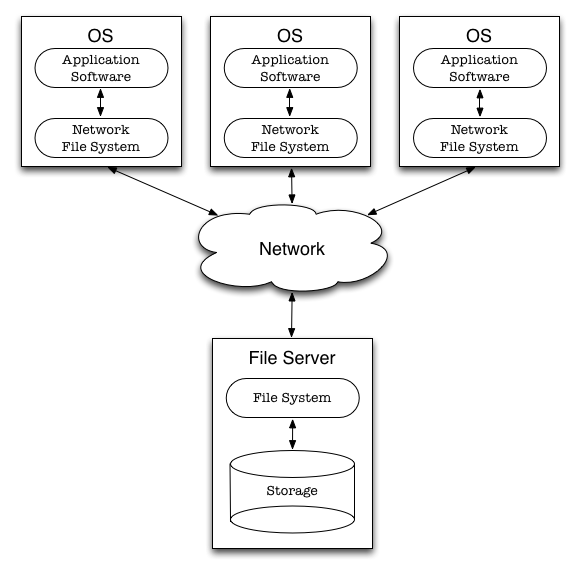
\includegraphics[width=.66\textwidth]{04/pics/nas}
		\caption{Three hosts using Network Attached Storage, or {\em NAS}
			\label{fig:storage:nas}}
\end{figure}


As the need for more and more data arises, we
frequently want to be able to access certain data from
multiple servers.  An old and still very common
example is to store all your users' data on shared
disks that are made available to all clients over the
network.  When a user logs into {\tt hostA}, she
expects to find all her files in place just as when
she logs into {\tt hostB}.  To make this magic happen,
two things are required: (1) the host's file system
has to know how to get the data from a central
location and (2) the central storage has to be
accessible over the network.  As you can tell, this
introduces a number of complex considerations, not the
least of which are access control and performance.

For the moment, let us put aside these concerns,
however, and look at the storage model from a purely
architectural point of view:  One host functions as
the ``file server'', while multiple clients access the
file system over the network.  The file server may be
a general purpose Unix system or a special network
appliance -- either way, it provides access to a
number of disks or other storage media, which, within
this system are effectively direct attached storage.
In order for the clients to be able to use the
server's file system remotely, they require support
for (and have to be in agreement with) the protocols
used\footnote{The most common protocols in use with
network attached storage solution are
\glslink{nfs}{NFS}\index{NFS} on the Unix side and
\glslink{smb}{SMB}\index{SMB}/\glslink{cifs}{CIFS}\index{CIFS}
on the Windows side.  The {\em Apple Filing Protocol}
(\glslink{afp}{AFP}\index{AFP}) is still in use in
some predominantly Mac OS environments, but Apple's
adoption of Unix for their Mac OS X operating system
made NFS more widespread there as well.}. However, the
clients do not require access to the storage media on
the block level; in fact, they {\em cannot} gain such
access.

From the clients' perspective, the job of managing
storage has become simpler:  I/O operations are
performed on the file system much as they would be on
a local file system, with the complexity of how to
shuffle the data over the network being handled in the
protocol in question.  This model is illustrated in
Figure \ref{fig:storage:nas}, albeit in a somewhat
simplified manner:  even though the file system is
created on the file server, the clients still require
support for the {\em network file system}\index{File
Systems!NFS}\glslink{nfs} that brokers the transaction
performed locally with the file server.

In contrast to \gls{das}, a dedicated file server
generally contains significantly more and larger
disks; \gls{raid} or \gls{lvm}\index{LVM} may likewise
be considered a requirement in this solution, so as to
ensure both performance and failover.  Given the
additional overhead of transferring data over the
network, it comes as no surprise that a certain
performance penalty (mainly due to network speed or
congestion) is incurred.  Careful tuning of the
operating system and in particular the network stack,
the TCP\glslink{tcp}\index{TCP} window size, and the
buffer cache can help minimize this cost.

The benefits of using a central file server for data
storage are immediate and obvious: data is no longer
restricted to a single physical or virtual host and
can be accessed (simultaneously) by multiple clients.
By pooling larger resources in a dedicated NAS device,
more storage becomes available.

Other than the performance impact we mentioned above,
the distinct disadvantage lies in the fact that the
data becomes unavailable if the network connection
suffers a disruption.  In many environments, the
network connection can be considered sufficiently
reliable and persistent to alleviate this concern.
However, such solutions are less suitable for mobile
clients, such as laptops or mobile devices, which
frequently may disconnect from and reconnect to
different networks.  Recent developments in the area
of {\em Cloud Storage\index{Cloud Storage}} have
provided a number of solutions (see Section \ref{file
systems:storage-models:cloud}), but it should be noted
that mitigation can also be found in certain older
network file systems and protocols: the {\em
\gls{afs}}\index{AFS}, for example, uses a local
caching mechanism that lets it cope with the temporary
loss of connectivity without blocking.

While network attached storage is most frequently used
for large, shared partitions or data resources, it is
possible to boot and run a server entirely without any
direct attached storage.  In this case, the entire
file system, operating system kernel and user data
may reside on the network.  We touch on this special
setup in future chapters.

\begin{figure}[!h]
	\subfloat[Huawei Tecal RH 2288H V2]{\label{fig:storage:nas-huawei}
			\raisebox{3em}{
				\includegraphics[width=.45\textwidth]{04/pics/huawei}}}
	\hspace{5em}
	\subfloat[NetApp FAS 3050c]{\label{fig:storage:san-netapp}
				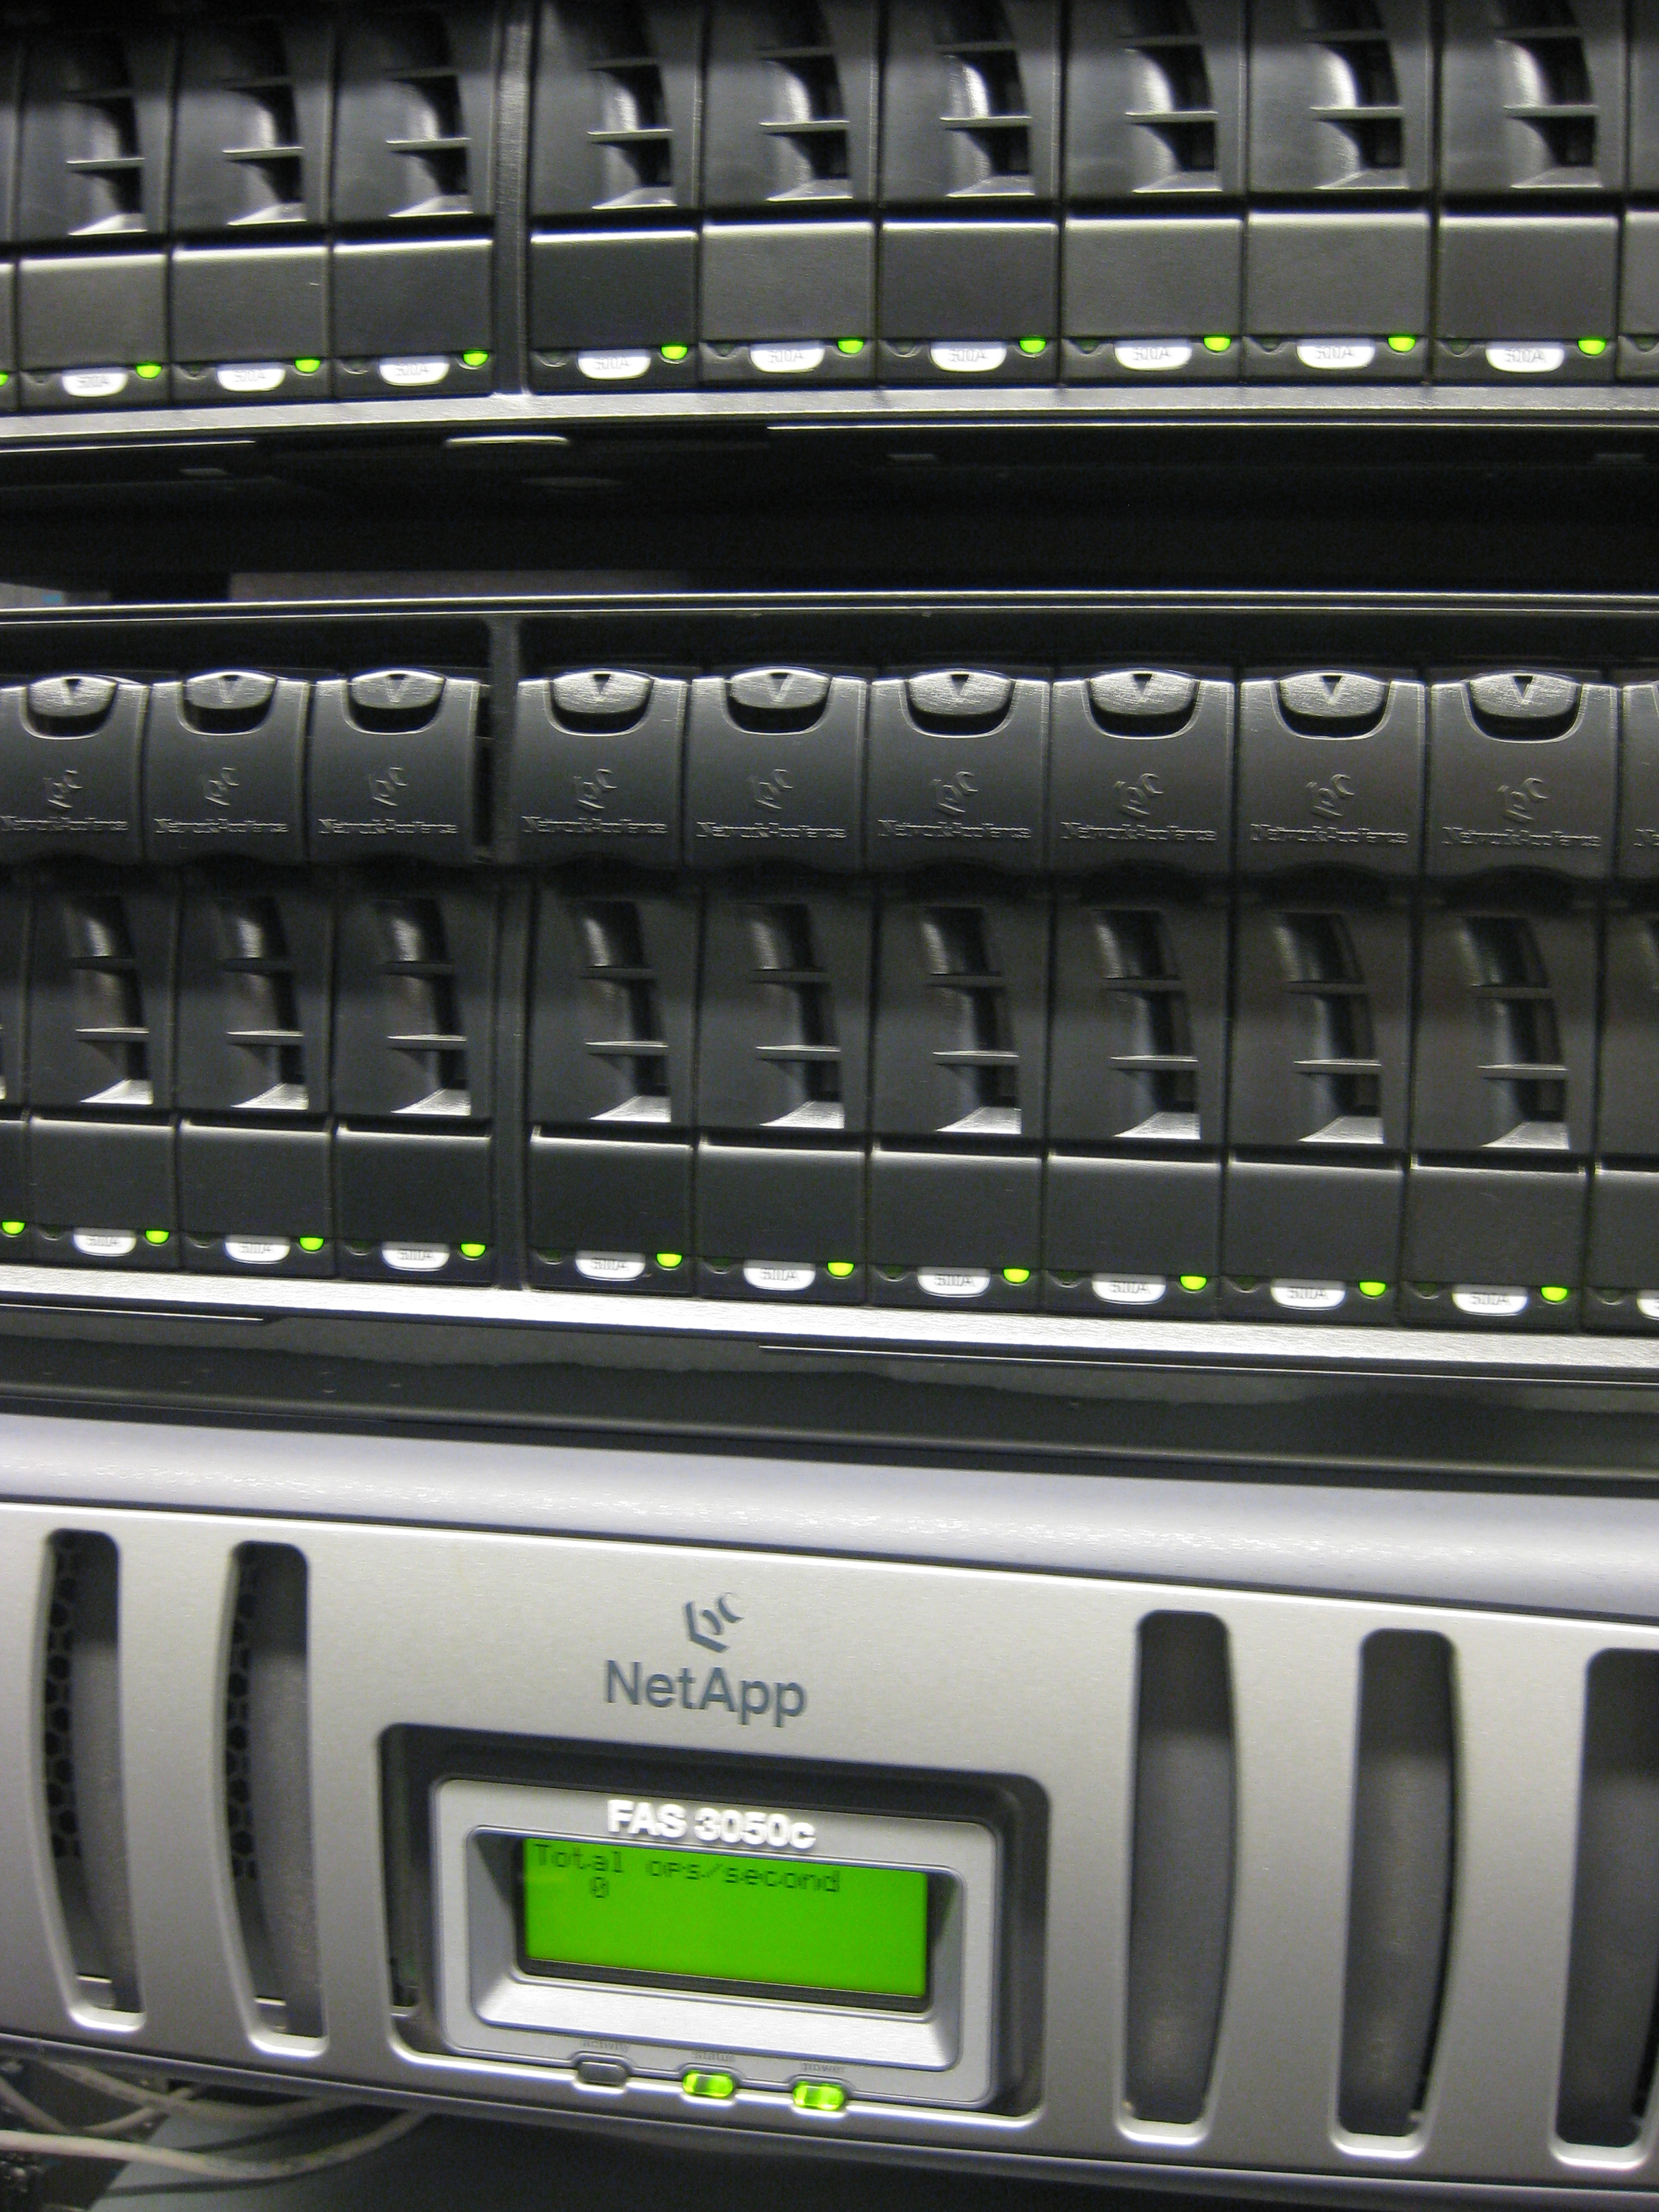
\includegraphics[width=.35\textwidth]{04/pics/netapp}}
	\caption{NAS and SAN Hardware}{NAS and SAN enterprise hardware.  On the left,
		Huawei storage servers with 24 hard
		drives each and built-in hardware RAID
		controllers; on the right, a NetApp
		Fabric Attached Storage device, also
		known as a ``filer'' with disk
		enclosures commonly referred to as ``shelves''.}
\end{figure}


\subsection{Storage Area Networks}
\label{file systems:storage-models:san}
\index{Storage Area Network}

\begin{figure}[ht]
	\centering
	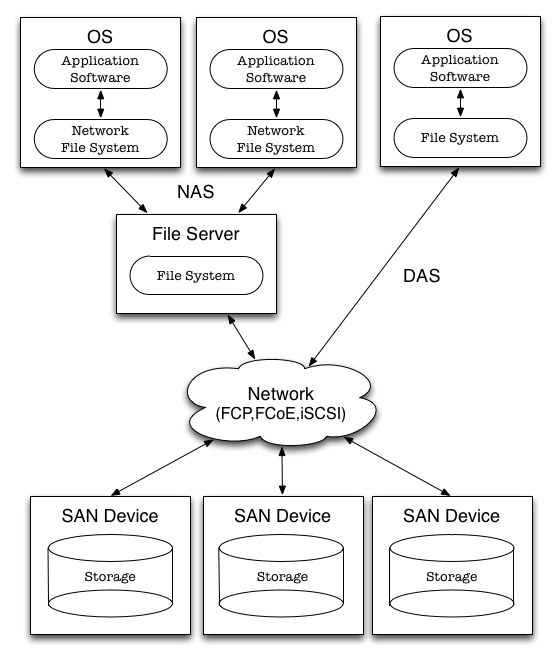
\includegraphics[width=.66\textwidth]{04/pics/san-nas-das}
		\caption[SAN illustrated]{A SAN providing access to three devices;
			one host accesses parts of the available storage
			as if it was DAS, while a file server manages
			other parts as NAS for two clients.
			\label{fig:storage:san}}
\end{figure}

\glsreset{nas}
\gls{nas} allows multiple clients to access the same file
system over the network, but that means it requires
all clients to use specifically this file system.  The
NAS file server manages and handles the creation of
the file systems on the storage media and allows for
shared access, overcoming many limitations of direct
attached storage.  At the same time, however, and
especially as we scale up, our requirements with
respect to storage size, data availability, data
redundancy, and performance, it becomes desirable to
allow different clients to access large chunks of
storage on a block level.  To accomplish this, we
build high performance networks specifically dedicated
to the management of data storage: {\em Storage Area
Networks}.\index{Storage Area Network}

In these dedicated networks, central storage media is
accessed using high performance interfaces and
protocols such as {\em Fibre Channel\index{Fibre
Channel}} or {\em iSCSI\index{iSCSI}}, making the
exposed devices appear local on the clients.  As you
can tell, the boundaries between these storage models
are not rigid: a single storage device connected via
Fibre Channel to a single host (i.e.  an example of
\gls{das}) is indistinguishable (to the client) from a
dedicated storage device made available over a
\gls{san}.  In fact, today's network file servers
frequently manage storage made available to them over
a \gls{san}\index{SAN} to export a file system to the clients as NAS.

Figure \ref{fig:storage:san} illustrates how the
storage volumes managed within a SAN can be accessed
by one host as if it was direct attached storage while
other parts are made available via a file server as
NAS to different clients.  In order for the different
consumers in a SAN to be able to independently address
the distinct storage units, each is identified by a
unique {\em \gls{lun}}.  The system administrator
combines the individual disks via RAID, for example,
into separate volumes; assigning to each storage unit
an independent LUN allows for correct identification
by the clients and prevents access of data by
unauthorized servers, an important security mechanism.
Fibre Channel switches used in SANs allow further
partitioning of the fabric by LUNs and subdivision
into SAN Zones\index{SAN Zones}, allowing sets of
clients specifically access to ``their'' storage
device only.

In this storage model the clients -- the computers,
file servers or other devices directly attached to the
SAN -- are managing the volumes on a block level (much
like a physical disk, as discussed in Section
\ref{sec:file-systems:physical-disk-structure}).  That is,
they need to create a logical structure on top of the
block devices (as which the SAN units appear), and
they control all aspects of the I/O operations down to
the protocol.  With this low-level access, clients can
treat the storage like any other device.  In
particular, they can boot off SAN attached devices,
they can partition the volumes, create different file
systems for different purposes on them and export them
via other protocols.

Storage area networks are frequently labeled an
``enterprise solution'' due to their significant
performance advantages and distributed nature.
Especially when used in a switched fabric,
additional resources can easily be made available to
all or a subset of clients.  These networks utilize
the {\em \gls{scsi}}\index{SCSI} protocol for communications
between the different devices; in order to build a
network on top of this, an additional protocol layer
-- the {\em \gls{fcp}}\index{Fibre
Channel!Protocol} being the most common
one -- is required. We will review the various
protocols and interfaces in Section \ref{file
systems:disk-devices-interface}.

SANs overcome their restriction to a {\em local} area
network by further encapsulation of the protocol: {\em
Fibre Channel over Ethernet}\index{Fibre Channel!over
Ethernet} (FCoE\index{Fibre Channel!over Ethernet}) or {\em
iSCSI}\index{iSCSI}, for example, allow connecting
switched SAN components across a Wide Area
Network\index{Wide Area Network} (or WAN).  But the
concept of network attached storage devices
facilitating access to a larger storage area network
becomes less accurate when end users require access to
their data from anywhere on the Internet.  Cloud
storage solutions have been developed to address these
needs.  However, as we take a closer look at these
technologies, it is important to remember that at the
end of the day, somewhere a system administrator is in
charge of making available the actual physical storage
devices underlying these solutions.  Much like a file
server may provide NAS to its clients over a SAN, so
do cloud storage solutions provide access on
``enterprise scale'' (and at this size the use of
these words finally seems apt) based on the foundation
of the technologies we discussed up to here.

\subsection{Cloud Storage}
\label{file systems:storage-models:cloud}
\index{Cloud Storage}

In the previous sections we have looked at storage
models that ranged from the very simple and very local
to a more abstracted and distributed approach, to a
solution that allows access across even a \gls{wan}.
At each step, we have introduced additional layers of
indirection with the added benefit of being able to
accommodate larger requirements: more clients, more
disk space, increased redundancy, etc.

We also have come full circle from direct attached
storage providing block-level access, to distributed
file systems, and then back around to block-level
access over a dedicated storage network.  But this
restricts access to clients on this specific network.
As more and more (especially smaller or mid-sized)
companies are moving away from maintaining their own
infrastructure towards a model of {\em
\gls{iaas}}\index{Infrastructure!As a Service} and
Cloud Computing\index{Cloud Computing}, the storage
requirements change significantly, and we enter the
area of {\em Cloud Storage}\footnote{Large companies are of
course also moving towards {\em IaaS}, only they
frequently are the ones simultaneously consuming as
well as {\em providing} the service, either internally
or to outside customers.}.

The term ``cloud storage'' still has a number of
conflicting or surprisingly different meanings.  On
the one hand, we have commercial services offering
{\em file hosting} or {\em file storage} services;
common well-known providers currently include Dropbox,
Google Drive, Apple's iCloud and Microsoft's SkyDrive.
These services offer customers a way to not only store
their files, but to access them from different devices
and locations: they effectively provide network
attached storage over the largest of WANs, the
Internet.

\begin{figure}[ht]
	\centering
	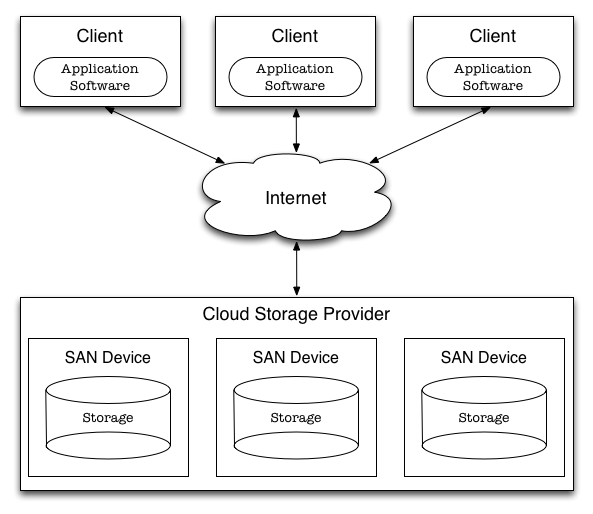
\includegraphics[width=.66\textwidth]{04/pics/cloud-storage}
		\caption[Cloud Storage]{A possible cloud storage model: an
			internal SAN is made available over the Internet to
			multiple clients.  In this example, the storage
			provider effectively functions as a NAS server,
			though it should generally be treated as a black box.
			\label{fig:storage:cloud}}
\end{figure}

On the other hand we have companies in need of a more
flexible storage solutions than can be provided with
the existing models.  Especially the increased use of
virtualization technologies demands faster and more
flexible access to reliable, persistent yet
relocatable storage devices.  In order to meet these
requirements, storage units are rapidly allocated from
large storage area networks spanning entire data
centers.

Since the different interpretations of the meaning of
``cloud storage'' yield significantly different
requirements, the implementations naturally vary, and
there are no current industry standards defining an
architecture.  As such, we are forced to treat each
product independently as a black box; system
administrators and architects may choose to use any
number of combinations of the previously discussed
models to provide the storage foundation upon which
the final solution is built.

We define three distinct categories within this
storage model: (1) services that provide file system
level access as in the case of file hosting services
such as those mentioned above; (2) services that
provide access on the {\em object level}, hiding file
system implementation details from the client and
providing for easier abstraction into an \gls{api} and
commonly accessed via web services\footnote{``Web
services'' generally expose an \gls{api} over HTTP or HTTPS
using \gls{rest}\index{REST} or the
\gls{soap}\index{SOAP}.} such as Amazon's
\gls{s3}\index{AWS!Simple Storage
Service}\index{AWS!S3}, or Windows Azure's {\em Blob}
Storage; and (3) services that offer clients access on
the block level, allowing them to create file systems
and partitions as they see fit (examples include
Amazon's \gls{ebs}\index{AWS!Elastic Block Store} and
OpenStack's\index{OpenStack} {\em Cinder} service).

All of these categories have one thing in common,
however.  In order to provide the ability of accessing
storage units in a programmatic way -- a fundamental
requirement to enable the flexibility needed in
demanding environments -- they rely on a clearly
specified \gls{api}.  Multiple distributed resources
are combined to present a large storage pool, from
which units are allocated, de-allocated, re-allocated,
relocated, and duplicated, all by way of higher-level
programs using well-defined interfaces to the
lower-level storage systems.

Customers of cloud storage solution providers reap a
wealth of benefits, including: their infrastructure is
simplified through the elimination of storage
components; storage units are almost immediately made
available {\em as needed} and can grow or shrink
according to immediate or predicted usage patterns;
applications and entire OS images can easily be
deployed, imported or exported as virtual appliances.

Of course these benefits carry a cost.  As usual, any
time we add layers of abstraction we also run the risk
of increasing, possibly exponentially, the number of
ways in which a system can fail.  Cloud storage is
no exception: by relying on abstracted storage
containers from a third-party provider, we remove the
ability to troubleshoot a system end-to-end; by
outsourcing data storage, we invite a number of
security concerns regarding data safety and
privacy\index{data privacy}; by accessing files over
the Internet, we may increase latency and decrease
throughput; the cloud service provider may become a
single point of failure for our systems, one that is
entirely outside our control.

\subsection{Storage Model Considerations}
\label{file systems:storage-models:considerations}

As we have seen in the previous sections, the larger
we grow our storage requirements, the more complex the
architecture grows.  It is important to keep this in
mind: even though added layers of abstraction and
indirection help us scale our infrastructure, the
added complexity has potentially exponential costs.
The more moving parts a system has, the more likely it
is to break, and the more spectacular its failure will
be.

A single bad hard drive is easy to replace; rebuilding
the storage array underneath hundreds of clients much
less so.  The more clients we have, the more important
it is to build our storage solution for redundancy as
well as reliability and resilience.

System administrators need to understand all of the
storage models we discussed, as they are intertwined:
\gls{das} must eventually underly any storage
solution, since the bits do have to be stored {\em
somewhere} after all; the concepts of NAS permeate any
infrastructure spanning more than just a few work
stations, and \gls{san}s\index{SAN} and cloud storage
combine DAS and NAS in different ways to make storage
available over complex networks.

At each layer, we introduce security risks, of which
we need to be aware: any time bits are transferred
over a network, we need to consider the integrity and
privacy of the files: who has access, who should
have access, how is the access granted, how are
clients authenticated, and so on.  NAS and SAN
solutions tend to ignore many of these implications
and work under the assumption that the network, over
which the devices are accessed, are ``secure''; access
controls are implemented on a higher layer such as the
implementation of the file system.  Often times,
access to the network in question implies access to
the shared storage, even though layer-2 security
mechanisms such as IPsec\index{IPsec}  may be combined
with or integrated into the solution.  Cloud storage,
on the other hand, has to directly address the problem
of transmitting data and providing access over
untrusted networks and thus usually relies on
application layer protocols such as
\gls{tls}\index{TLS}/\gls{ssl}\index{SSL}.

We will touch on some of these aspects in future
sections and chapters, but you should keep them in
mind as you evaluate different solutions for different
use cases.  As we will see, in most cases the simpler
model turns out to be the more scalable and more
secure one as well, so beware adding unneeded layers
of complexity!


\section{Disk Devices and Interfaces}
\label{file systems:disk-devices-interface}

\begin{figure}[t]
	\centering
	\subfloat[Open Hard Disc Drive]{\label{fig:file-systems:open-hard-drive}
			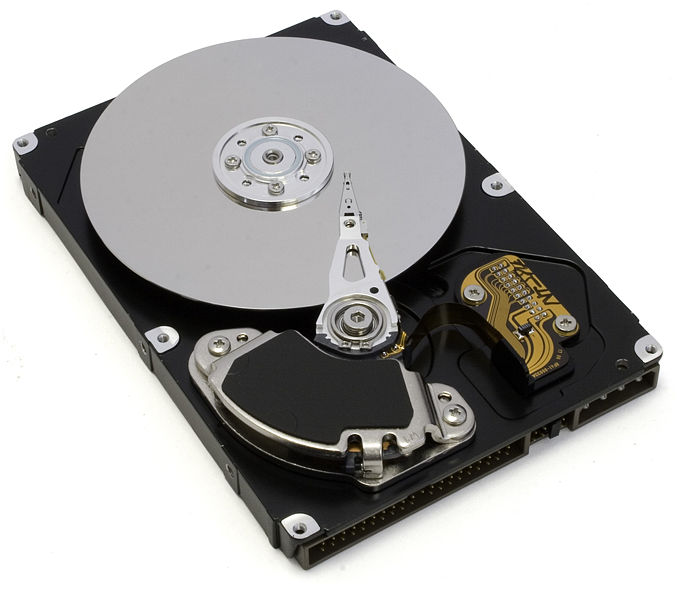
\includegraphics[width=.4\textwidth]{04/pics/open-hard-drive}}
	\hspace{7em}
	\subfloat[SSD Mini PCIe Card]{\label{fig:file-systems:ssd-mini-pcie}
			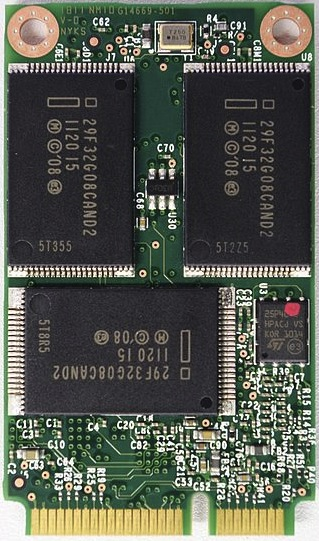
\includegraphics[width=.2\textwidth]{04/pics/ssd-minipcie}}
	\caption[HDD vs. SSD]{An open PATA (or IDE) hard drive (left) and
			a Solid State Drive (right).
			The HDD shows the rotating disk platters, the read-write
			head with its motor, the disk controller and
			the recognizable connector socket.
			\label{fig:file-systems:hdd-vs-ssd}}
\end{figure}



The different storage models we discussed in the
previous sections are just a means to access the
storage devices in order to, well, store our data.
Devices or media used to store data include tape
drives (for use with magnetic tape), optical media
such as CDs, various non-volatile memory based devices
such as flash drives,
\glslink{dram}{DRAM}\index{DRAM}-based storage, and of
course the \glslink{hdd}hard-disk drive
(HDD\index{HDD}).

Even though \gls{sdd}\index{SDD} offer significant
advantages such as lower power consumption and
generally higher performance, the dominant medium in
use especially in enterprise scale storage solutions
remains the ubiquitous hard drive\footnote{Despite
declining prices for SDDs, as of 2012 traditional hard
drives remain notably cheaper than SSDs and have
higher storage capacity.}, storing data on rotating,
magnetic platters (see Figure
\ref{fig:file-systems:open-hard-drive}).
Understanding the physical structure of these
traditional storage devices is important for a system
administrator, as the principles of especially the
addressing modes and partition schemas used here come
into play when we look at how file systems manage data
efficiently.

Hard drives can be made available to a server in a
variety of ways.  Individual disks are connected
directly to a \gls{hba}\index{Host Bus Adapter} using
a single data/control cable and a separate power
cable.  The traditional interfaces here are
\gls{scsi}\index{SCSI}, \glslink{pata}{PATA}\index{PATA} and
\glslink{sata}{SATA}\index{SATA}, as well as Fibre
Channel\index{Fibre Channel}.

SCSI, the {\em Small Computer System Interface}, has
been around for over 25 years and has seen a large
number of confusing implementations and
standards\footnote{Different SCSI versions include
such wonderful variations as {\em Fast SCSI}, {\em
Fast Wide SCSI}, {\em Ultra SCSI}, and {\em Wide Ultra
SCSI}. None of which are to be confused with {\em
iSCSI}, of course.}.  Once the default method to
connect any peripheral device using long, wide and
generally unwieldy ribbon cables, SCSI has now been
largely obsoleted by the {\em Advanced Technology
Attachment} (ATA\index{ATA}) standards.  At the same
time, however, it lives on in the {\em Internet Small
Computer System Interface} ({\em iSCSI\index{iSCSI}}),
a standard specifying storage connections using the
SCSI command protocol over IP-based networks.  iSCSI
is a common choice in storage area networks; as it
uses TCP/IP\index{TCP/IP} over existing networks, it
does not require a dedicated storage network as is the
case in traditional Fibre Channel SANs.

The {\em \gls{pata}} standard, also frequently
referred to as IDE\index{IDE} (for {\em Integrated
Device Electronics}, a reference to the fact that the
drive controller is included in the hard drive), uses
a 40 or 80 wire ribbon cable and allows for a maximum
number of two devices on the connector (traditionally
referred to as the {\em master} and {\em slave}; this
is often a source of confusion, as neither device
takes control or precedence over the other).

Faster throughput, smaller cables and support for
hot-swapping\index{hot swapping}, i.e. the ability to replace a drive
without having to shut down the operating
system\footnote{Hot-swapping was a standard feature in
many SCSI implementations.  Many system administrators
in charge of the more powerful servers, using larger
and more performant SCSI drives when compared to the
individual workstations at the time, were rather fond
of this: when a disk failed, it could be replaced
without scheduling downtime for {\em all} services.},
were some of the advantages provided by the {\em
Serial ATA} (\glslink{sata}{SATA}\index{SATA})
interface.  A number of revisions and updates to the
standard added more advanced features and, most
significantly, increasingly greater transfer speeds.

Most motherboards have integrated ATA host adapters,
but a server can be extended with additional
\glslink{hba}{HBAs} via, for example, its
\glslink{pci}{PCI} Express\index{PCI Express}
expansion slots; similarly, dedicated storage
appliances make use of disk array controllers to
combine multiple drives into logical units (more on
that in Section \ref{file
systems:storage-models:dividing-and-combining-disks}).
Fibre Channel HBAs finally allow a server to connect
to a dedicated Fibre Channel\index{Fibre Channel!SAN}
SAN.  All of these interfaces can be either internal
(the devices connected to the bus are housed within
the same physical enclosure as the server) or external
(the devices are entirely separate of the server,
racked and powered independently and connected with
suitable cables).  In the end, consider a host with a
large amount of \gls{das} and a NAS server managing
multiple terabytes of file space which is housed in
a separate device and which it accesses over a SAN:
the main difference lies not in the technologies and
protocols used, but in how they are combined. \\

\begin{advice}
{\bf Hands-on Hardware} \\
I have found it useful to have actual hardware in
class whenever possible.  In the past, I have brought
with me different hard drives by different
manufacturers and with different interfaces (PATA,
SATA, SCSI); in particular, showing students the
inside of a hard drive, the rotating platters and the
read-write arms has served as a great illustration of
the performance limiting factors, such as rotational
latency, seek time etc.  Especially old and by now
possibly obsolete hardware and the contrast in which
it stands to modern solutions is always investigated
with great interest. \\[10pt]

Likewise, a large variety of cables, connectors and
adapters help illustrate the different standards and
allow students to connect what they may have seen or
used themselves to what we talk about in class.  (See
also: Problem \ref{prob:disks:hdds})
\end{advice}

\subsection{Physical Disk Structure}
\label{sec:file-systems:physical-disk-structure}

Let us open up a typical hard drive and take a look at
the physical structure.  This will help us better
understand the concepts of partitions, how the
operating system calculates the disk geometry and
allocates physical blocks, how the file system manages
cylinder groups\index{cylinder groups}, and why, for
example, storing data on the outer disk blocks could
improve performance.

If you open a traditional hard-disk drive and manage
not to destroy it completely in the process, you will
look at a number of magnetic platters on a spindle
together with the read-write heads.  The other main
components include the disk motor (spinning the
platters), an actuator (moving the read-write heads)
and the disk controller.

The platters are coated on both surfaces with magnetic
particles, allowing us to store on (and retrieve off)
them data in the form or zeros and ones by polarizing
the relevant area.  The read-write heads -- one for
each platter surface -- may be resting on the {\em
landing zone} near the spindle; they do not touch the
platters when they are rotating.  Instead, they hover
just above the platters and are moved radially across
the disks by the actuator to position them at the
desired location.  If the read-write heads are brought
into contact with the spinning platters, the results
tend to be rather disastrous, as the magnetic surface
of the disk is damaged by this {\em head
crash}\index{head crash}.

\begin{figure}[ht]
	\centering
	\subfloat[Disk Structure: Cylinders/Tracks, Heads, Sectors]{
			\label{fig:file-systems:chs}
			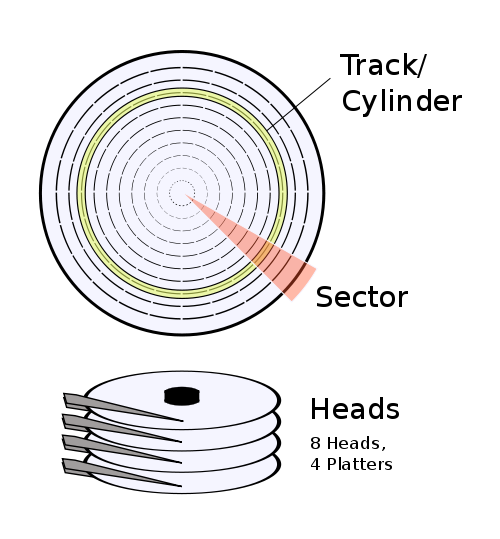
\includegraphics[width=.4\textwidth]{04/pics/chs}}
	\hspace{1em}
	\subfloat[Physical Disk Structure with Zone Bit Recording]{
			\label{fig:file-systems:disk-structure-zbr}
			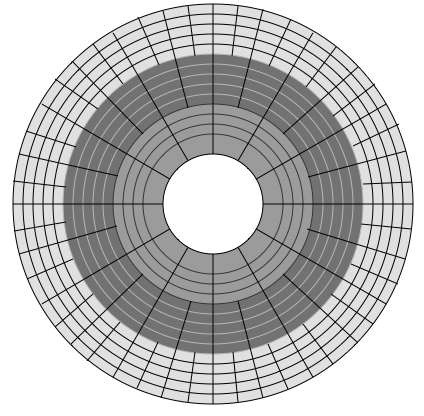
\includegraphics[width=.4\textwidth]{04/pics/disk-structure-zone-bit-recording}}
	\caption[Physical Disk Structure]{On the left: Illustration of tracks and sectors
			on a hard disk.  Note that for simplicity,
			sectors on the inside and outside
			of the platters are of identical size.  On
			disks with Zone Bit Recording\index{Zone Bit Recording}
			(shown on the right), this is no longer the case.}
\end{figure}


The surface of each platter is divided into concentric
rings, or {\em tracks}.  Congruent tracks on multiple
platters form a three-dimensional {\em cylinder}.
Within a single cylinder, data can be read from all
available surfaces without requiring the read-write
heads to move.  This is why {\em disk
partitions}\index{partition} comprise multiple
cylinder groups\index{cylinder groups} rather than, as
we may sometimes imagine them to be, pie wedges.


The tracks on each platter are in turn divided into a
number of {\em sectors}.  If you were to divide a disk
with concentric tracks by drawing straight lines from
the center to the outer edge, you would quickly
realize that even though you end up with the same
number of such sectors on each track, the fields
created in this manner would be of varying sizes:  the
ones on the outer edge would be significantly larger
than the ones in the middle of the disc (see Figures
\ref{fig:file-systems:chs} and
\ref{fig:file-systems:disk-structure-zbr}).

As these fields represent the smallest addressable
unit on a hard drive, we would be wasting a lot of
disk space.  Instead, each sector is kept at a fixed
size\footnote{The industry standard for hard drives
used to be 512 bytes for many years; since around
2010, a number of vendors have started creating hard
drives with a physical block size of 4096 bytes.
Interestingly, file systems having standardized on 512
byte blocks tend to divide these blocks and continue
to present to the OS 512 byte ``physical'' blocks.}
and use a technique known as {\em Zone Bit
Recording}\index{Zone Bit Recording} to store more
sectors on the outer tracks of each disc than on the
inner area.

The total number of 512 byte sectors across all
platters of the hard drive thus define its total
capacity.  In order to access each storage unit, the
read-write head needs to be moved radially to the
correct cylinder -- a process we call {\em seeking} --
and the platter then spun until the correct sector is
positioned under it.  In the worst case scenario, we
just passed the sector we wish to access and we have
to perform a full rotation.  Therefore, a drive's
performance is largely defined by this {\em rotational
latency}\index{rotational latency} and the time to
position the read-write head (also known as {\em seek
time}).

Since the motor of a drive may rotate the discs at a
constant linear velocity (versus constant angular
velocity), the discs are in fact moving slower near
the spindle than on the outer part.  This means that
more sectors could be read in a given time frame from
the outside of the discs than from the inside.  In
fact, it used to be not uncommon for system
administrators to partition their disks such that
large, frequently accessed files would reside on
cylinders near the beginning (i.e. the outside) of the
platters.  Nowadays such fine tuning may no longer be
common, but instead people have started to simply
create a single partition occupying only about 25\% of
the disk at the beginning and ignoring the rest.  This
technique, known as ``{\em short stroking}\index{short
stroking}'', may seem wasteful, but the performance
gain compared to the cheap prices of today's HDDs may
make it actually worthwhile.

It is worth noting that the physical disk structure
described here applies only to traditional mechanical
hard drives, not to Solid State Drives\index{Solid
State Drive} or other storage media.  Nevertheless, it
is useful to understand the structure, as a number of
file system or partitioning conventions derive
directly from these physical restrictions.

\begin{sidenote}
{\bf True Hard Drive Capacity} \\
Hard drive manufacturers use a different definition of
what constitutes a Gigabyte than is customary pretty
much anywhere else: normally, we define computer
storage in terms of powers of two.  That is, a
kilobyte is commonly understood to be $2^{10}$ bytes,
a megabyte $2^{20}$ and a gigabyte $2^{30}$.  In
contrast, the standard prefix {\em giga} means $10^9$,
and hard drive manufacturers use this meaning.  Some
people differentiate between these conflicting
definitions by using the term {\em Gibibyte} (GiB) for
$2^{30}$ bytes, but even though technically correct,
this term has never really caught on. \\[10pt] As a
result, a drive labeled as having a capacity of 500 GB
will in fact only be able to store around 465 GiB.
The larger the drive, the bigger the difference - at
1TB ($2^{40}$ versus $10^{12}$), you are getting a
full 10\% less storage than advertized!
\end{sidenote}

\section{Dividing and Combining Disks}
\label{file systems:storage-models:dividing-and-combining-disks}

Disk space is a finite and fixed resource.  Each hard
drive we purchase has a given capacity, and it is up
to the system administrators to use it efficiently.
In this section, we will take a look at the
different methods to provide the optimal amount of
storage space to your systems.  Sometimes this
involves dividing a single hard drive into multiple
partitions; other times, we want to combine multiple
hard drives to increase capacity, yet retain a logical
view of the storage space as a single unit.  Finally,
the ways in which we divide or combine disks have
implications on system performance and data
redundancy.



\subsection{Partitions}
\label{file systems:storage-models:dividing-and-combining-disks:partitions}
\index{Disks!Partitions}

Now that we understand the physical layout of the hard
disks, we can take a look at how we {\em partitions}
are created and used.  As we noted in the previous
section, a disk partition is a grouping of adjacent
cylinders through all platters of a hard
drive\footnote{Some operating systems such as Solaris,
for example, have traditionally referred to partitions
as ``slices''; some of the BSD systems also refer to
disk ``slices'' within the context of {\em
\glslink{bios}{BIOS} partitions}.  Unfortunately, this
easily brings to mind the misleading image of a slice
of pie, a wedge, which misrepresents how partitions
are actually laid out on the disk.}.  Despite this
unifying principle, we encounter a variety of
partition types and an abundance of related
terminology: there are {\em partition
tables\index{partition!table}} and {\em disklables},
{\em primary}\index{partition!primary} and {\em
extended}\index{partition!extended} partitions; there
are whole-disk partitions, disks with multiple
partitions, and some of the partitions on a disk may
even overlap.

Different file systems and anticipated uses of the
data on a disk require different kinds of partitions.
First, in order for a disk to be bootable, we require
it to have a {\em boot sector}\index{boot sector}, a
small region that contains the code that the
computer's firmware (such as the
\gls{bios}\index{BIOS}) can load into memory.  In
fact, this is precisely what a BIOS does: it runs
whatever code it finds in the first sector of the
device so long as it matches a very simple boot
signature\index{boot signature}.  That is, regardless
of the total capacity of the disk in question, the
code that chooses how or what to boot needs to fit
into a single sector, 512 bytes.  On most commodity
servers\footnote{Even though many other hardware
architectures used to be dominant in the server
market, nowadays the {\em x86} instruction set (also
known as ``IBM PC-compatible'' computers) has replaced
most other systems.  For simplicity's sake, we will
assume this architecture throughout this chapter.},
this code is known as the {\em Master Boot
Record}\index{Master Boot Record} or MBR.  In a
classical MBR the bootstrap code area itself takes
up 446 bytes and each partition entry requires 16
bytes.  As a result, we can have at most four such
{\em BIOS partitions}\index{Partitions!BIOS} that the
MBR can transfer control to.

\begin{lstlisting}[float,label=code:fdisk,caption=fdisk(8) sample invocation
and output on a Linux system]
# fdisk -l
Disk /dev/cciss/c0d0: 73.3 GB, 73372631040 bytes
255 heads, 63 sectors/track, 8920 cylinders
Units = cylinders of 16065 * 512 = 8225280 bytes

           Device Boot Start   End    Blocks   Id  System
/dev/cciss/c0d0p1   *      1  2550  20482843+  83  Linux
/dev/cciss/c0d0p2       2551  7649  40957717+  83  Linux
/dev/cciss/c0d0p3       7650  7904   2048287+  82  Linux swap
#
\end{lstlisting}

Sometimes you may want to divide the available disk
space into more than four partitions.  In order to
accomplish this, instead of four {\em primary}
partitions, the MBR allows you to specify three
primary and one so-called {\em extended} partition,
which can be subdivided further as needed.  When the
system boots, the \gls{bios} will load the MBR code, which
searches its partition table for an ``active''
partition, from which it will then load and execute
the boot block.  This allows the user to run multiple
operating systems from the same physical hard drive,
for example.  BIOS partitions are usually created or
maintained using the {\tt fdisk(8)}\index{\tt fdisk(8)}
utility.

\begin{sidenote}
{\bf Disk and BIOS Limitations} \\

In order to address sectors of a hard drive, computers
used the {\em
\gls{chs}}\index{Addressing!Cylinder-Head-Sector}
scheme.  Early BIOSes were only able to address 1024
cylinders, 256 heads and 63 sectors/track.  At the
same time, the ATA specification for IDE disks defined
a limit of 65536 cylinders, 16 heads, and 256 sectors.
As a result, the lowest common denominator required
addressing -- and thus total disk sizes -- to be
limited to:\\ [10pt]

$1024 (cylinders) * 16 (heads) * 63 (sectors) * 512 (bytes / sector) = 504 MB $ \\[10pt]

{\em Enhanced BIOS}es removed some of these
limitations, allowing for disks with an at that time
impressive size of approximately 8 GB ($1024 * 255 *
63 * 512$).  But they were only able to access the
first 1024 cylinders of a disk.  This meant that all
the files required to boot the OS (which then might be
able to address more disk space) had to reside within
these cylinders.  As a result, many Unix systems have
a default partitioning scheme including a small {\tt
/boot} partition created at the beginning of the disk.
\\ [10pt]

To overcome the limitations of
\gls{chs}\index{Addressing!Cylinder-Head-Sector}
addressing, data blocks on the disks were simply
numbered and counted, yielding {\em
\gls{lba}}\index{Addressing!Logical Block}.  Using
this method, IDE disks could thus address however many
blocks it could store in the data type it used for
this purpose; the ATA specification used 28 bits, and
thus imposed a limit of $(2^{28}\,sectors * 512\,
bytes/sector)/1024^3\, bytes/GB = 128\, GB$ (or
$~137.4GiB$ at $10^9\, bytes/GiB$). \\ [10pt]

In 2012, the current ATA/ATAPI\index{ATA}
specification uses 48 bits, limiting disk size to 128
Petabytes (PB); however, some operating systems still
use 32 bits to address sectors, so that on those
systems the largest supported disk size is 2 Terabyte
(TB), yet another limitation we now run into and which
may seem laughably small in just a few years.
\end{sidenote}


Just as the first sector of the disk contains the MBR,
so does the first sector of a \gls{bios} partition
contain a {\em volume boot record}\index{volume boot
record}, also known as a {\em partition boot
sector}\index{partition boot sector}.  In this sector,
the system administrator may have placed a
second-stage bootloader\index{bootloader}, a small
program that allows the user some control over the
boot process by providing, for example, a selection of
different kernels or boot options to choose from.
Only one partition is necessary to boot the OS, but
this partition needs to contain all the libraries and
executables to bootstrap the system.  Any additional
partitions are made available to the OS at different
points during the boot process.

\begin{lstlisting}[basicstyle=\scriptsize,float,label=code:disklabel,caption=disklabel(8)
invocation and output on a NetBSD system]
# dmesg | grep xbd3
xbd3 at xenbus0 id 3: Xen Virtual Block Device Interface
xbd3: 24575 MB, 512 bytes/sect x 50331520 sectors
# disklabel /dev/xbd3
type: ESDI
disk: Universal Swap
label: disk1
bytes/sector: 512
sectors/track: 306432
tracks/cylinder: 1
sectors/cylinder: 306432
cylinders: 255
total sectors: 78140160
rpm: 3600
interleave: 1

8 partitions:
#      size   offset fstype [fsize bsize cpg/sgs]
a: 20972385       63 4.2BSD   4096 32768    1180  # (Cyl.     0*- 20805)
b:  1048320 20972448   swap                       # (Cyl. 20806 - 21845)
c: 78140097       63 unused      0     0          # (Cyl.     0*- 77519)
d: 78140160        0 unused      0     0          # (Cyl.     0 - 77519)
e: 56119392 22020768 4.2BSD   4096 32768   58528  # (Cyl. 21846 - 77519)
#
\end{lstlisting}


In the BSD family of operating systems, the volume
boot record contains a {\em disklabel}, detailed
information about the geometry of the disk and the
partitions it is divided into.  Listing
\ref{code:disklabel} shows the output of the {\tt
disklabel(8)}\index{\tt disklabel(8)} command on a
NetBSD\index{NetBSD} system.  You can see the
breakdown of the disk's geometry by cylinders, sectors
and tracks and the partitioning of the disk space by
sector boundaries.  This example shows a 40
GB\footnote{$ (78140160\, sectors * 512\, bytes/sector) /
(1024^3\, bytes/GB) = 37.26\, GB$ \\ Note the difference
in actual versus reported disk size: \\ $(40*2^{30} -
40*10^9)/(1024^3) = 40 - 37.26 = 2.74$ } disk
containing three partitions, a 10 GB root partition, a
512 MB swap partition and a data partition comprising
the remainder of the disk.  Since the disk in question
is actually a virtual disk, the information reported
relating to the hardware, such as the {\tt rpm} rate,
for example, is obviously wrong and should be ignored.
This serves as a reminder that a system
administrator always may need to have additional
background knowledge (``this host is a virtual machine
with a virtual disk'') to fully understand the output
of her tools in order to make sense of it.  Note also
that some partitions overlap.  This is not a mistake:
the BSD disklabel includes information about both the
entire disk (partition '{\tt d}') as well as the
\gls{bios} partition assigned to NetBSD (partition '{\tt
c}', starting at offset {\tt 63}).  Other partitions,
i.e.  partitions actually used by the OS, should {\em
not} overlap.

Being able to read and understand the detailed output
of these commands is important, and students are
encouraged to practice making sense of different
partition schemas across different operating systems
(see exercise \ref{prob:disks:disklabel}). \\

Dividing a single large disk into multiple smaller
partitions is done for a number of good reasons: if
you wish to install multiple operating systems, for
example, you need to have dedicated disk space as well
as a bootable primary partition for each OS.  You may
also use partitions to ensure that data written to one
location (log files, for example, commonly stored
under e.g. {\tt /var/log}) cannot cause you to run out
of disk space in another (such as user data under {\tt
/home}).  Other reasons to create different partitions
frequently involve the choice of file system or mount
options, which necessarily can be applied only on a
per-partition basis.  We will discuss a number of
examples in Section \ref{sec:file systems}.

\subsection{Logical Volumes}
\label{file systems:storage-models:dividing-and-combining-disks:logical-volumes}
\index{Logical Volumes}

Using hard drives with fixed partitions may lead to a
number of problems: disk drives are prone to hardware
failure, which may lead to data loss; reading data
from individual disk drives may suffer performance
penalties depending on the location of the data on the
disk; and, perhaps most notably, disks are never large
enough.

Partitions are a good way to divide a single disk and
make available to the OS smaller, distinct units of
storage.  But throughout the life time of our systems,
we frequently have a need to {\em increase} storage
space -- consider the quote from the beginning of this
chapter: ``{\em Data expands to fill any void.}''  We
can buy a larger hard drive and add it to the system
and then migrate data to it or simply mount it in a
separate location\footnote{An approach aptly
described as ``\glslink{jbod}{JBOD}\index{JBOD}'':
``Just a Bunch Of Disks''.}, but neither solution is
particularly elegant.  The problem here is that
partitions are fixed in size throughout their life
time.  Wouldn't it be nice if we could simply combine
the storage from multiple disk drives and then create
partitions spanning the total?

Enter {\em logical volumes}.  Much like a
\gls{san}\index{SAN} may combine multiple storage
devices and make them available to its clients, so
does a logical volume manager (or
\gls{lvm}\index{LVM}) combine multiple physical
devices and present them to the OS as a single
resource.  In this case, the abstraction occurs on the
device-driver level; some advanced file systems may
include aspects of an LVM (see ZFS\index{ZFS}'s
\manpage{zpool(1)} command, for example).

\begin{figure}[ht]
	\centering
	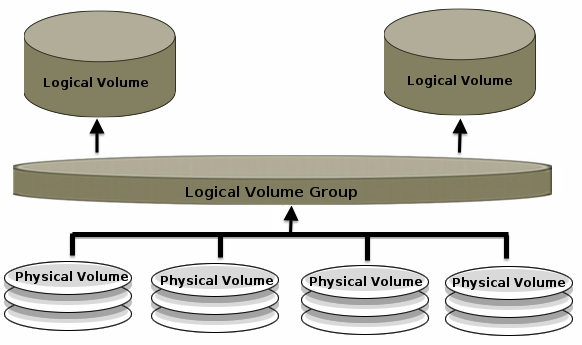
\includegraphics[width=.75\textwidth]{04/pics/lvm}
		\caption[Logical Volume Management]{Logical Volume
			Management lets you combine multiple physical disks
			or partitions into a single {\em volume group},
			from which {\em logical volumes} can be allocated.
			\label{fig:file-systems:lvm}}
\end{figure}



The management of the locally attached storage devices
via so-called {\em logical volume groups} grants the
system administrator a significant amount of
flexibility: the total storage space can
easily be extended (and the file system, if it
supports this operation, grown!) by adding new disk
drives to the pool; file system performance can be
improved by {\em striping} data across all available
drives; data redundancy and fault tolerance can be
improved by {\em mirroring} data on multiple devices.
These last two advantages are also provided by the
\gls{raid} storage solution, which we will look at in more
detail in the following section. \\

\gls{lvm}s manage and combine three distinct
resources, as illustrated in Figure
\ref{fig:file-systems:lvm}: {\em physical volumes},
{\em logical volume groups} and {\em logical volumes}.
A physical volume can be a hard disk, a partition on a
hard disk, or a logical unit number of a local or
remote device (such as SAN connected storage device).
The LVM divides the physical volumes into data blocks,
so-called {\em physical extents}\index{LVM!physical
extent}, and allows the system administrator to group
one or more of these physical volumes into a logical
volume group.  In effect, available storage space is
combined into a pool, where resources can dynamically
be added or removed.  Out of such a volume group,
individual logical volumes can then be created, which
in turn are divided into the equivalent of a hard
disk's sectors, so-called {\em logical
extents}\index{LVM!logical extent}.  This step of
dividing a logical volume group into logical volumes
is conceptually equivalent to the division of a single
hard drive into multiple partitions; in a way, you can
think of a logical volume as a virtual disk.  To the
operating system, the resulting device looks and
behaves just like any disk device: it can be
partitioned, and new file systems can be created on
them just like on regular hard drive disks.

By creating logical extents as storage units on the
logical volumes, the LVM is able to grow or shrink
them with ease (the data corresponding to the logical
extends can easily be copied to different physical
extents and remapped), as well as implement data
mirroring (where a single logical extent maps to
multiple physical extents).

Since logical volume management is a software solution
providing an additional layer of abstraction between
the storage device and the file system, it can provide
additional features both on the lower level, such as
data mirroring or striping, as well as on a higher
level, such as file system snapshots\index{snapshots},
which an \gls{lvm} can easily implement using a
``copy-on-write''\index{Copy-on-Write} approach when
updating the logical extents.  We will discuss this
topic in more detail in our chapter on backups in
Section \ref{backup:file-system-backups}.

Note that some of the desirable features of logical
volume management are not entirely independent of the
higher file system layer.  For example, a change in
size of the logical volumes requires the file system
to adapt, and growing a file system to expand to
consume additional disk space is often easier than
shrinking the file system.  Hence, the choice to use
an \gls{lvm} needs to be coupled with the ``right'' file
system!

\subsection{RAID}
\label{file systems:storage-models:dividing-and-combining-disks:raid}
\index{RAID}

Logical Volume Managers provide a good way to
consolidate multiple disks into a single large storage
resource from which individual volumes can be created.
An \gls{lvm} may also provide a performance boost by
striping data, or redundancy by mirroring data across
multiple drives.

Another popular storage technology used for these
purposes is {\em RAID}, which stands for {\em
Redundant Array of Independent Disks}\footnote{The
acronym ``\gls{raid}'' is sometimes expanded as ``Redundant
Array of {\em Inexpensive} Disks''; since disks have
become less and less expensive over time, it has
become more customary to stress the ``independent''
part.  A cynic might suggest that this change in
terminology was driven by manufacturers, who have an
interest in not explicitly promising a low price.}.
Multiple disks can be combined in a number of ways to
accomplish one or more of these goals: (1) increased
total disk space, (2) increased performance, (3)
increased data redundancy.

Much like an \gls{lvm}, RAID as well hides the
complexity of the management of these devices from the
OS and simply presents a virtual disk comprised of
multiple physical devices.  However, unlike with
logical volume management, a RAID configuration cannot
be expanded or shrunk without data loss.  Furthermore,
an \gls{lvm}is a software solution; RAID can be
implemented on either the software or the hardware
layer.  In a hardware RAID\index{RAID!Hardware}
solution, a dedicated disk array controller (such as a
PCI\glslink{pci} card) is installed in the server, and
interacted with via controlling firmware or host-level
client tools.  As a software implementation, an
\gls{lvm} may provide RAID\index{RAID!Software}
capabilities, as may certain file systems.  {\em
ZFS}\index{ZFS}, originally developed at Sun
Microsystems\index{Sun Microsystems}, for example,
includes subsystems that provide logical volume
management and offer RAID capabilities, as does
Linux's {\em Btrfs}\index{Btrfs}\index{B-tree file
system}.

When combining disks in a RAID configuration, the
system administrator has to carefully consider the
advantages and disadvantages of the available options,
so-called {\em RAID levels}, where performance,
redundancy, and efficiency of disk usage need to be
weighed.  The common RAID levels are summarized in
Table \ref{table:file systems:raid-std} (although many
more combinations and obscure levels exist); the by
far most popular levels are: {\em RAID 0}, {\em RAID
1} and {\em RAID 5}.

\begin{table}[ht]
\centering
	\begin{tabular}{ l p{.75\textwidth}}
	\hline
	{\bf RAID 0} & Striped array (block level), no parity or mirroring \\
	{\bf RAID 1} & Mirrored array, no parity or striping \\
	{\bf RAID 2} & Striped array (bit level) with dedicated parity \\
	{\bf RAID 3} & Striped array (byte level) with dedicated parity \\
	{\bf RAID 4} & Striped array (block level) with dedicated parity \\
	{\bf RAID 5} & Striped array (block level) with distributed parity \\
	{\bf RAID 6} & Striped array (block level) with double distributed parity \\
	\hline
	\end{tabular}
	\caption{A brief summary of standard RAID levels.}
	\label{table:file systems:raid-std}
\end{table}


\subsubsection{RAID 0}
\index{RAID!Level 0}

By writing data blocks in parallel across all
available disks (see Figure
\ref{fig:file-systems:raid-0}), RAID 0 accomplishes a
significant performance increase.  At the same time,
available disk space is linearly increased (i.e. two
500 GB drives yield 1 TB of disk space, minus
overhead).  However, RAID 0 does not provide any fault
tolerance: any disk failure in the array causes data
loss.  What's more, as you increase the number of
drives, you also increase the probability of disk
failure.

\subsubsection{RAID 1}
\index{RAID!Level 1}

This configuration provides increased fault tolerance
and data redundancy by writing all blocks to all disks
in the array, as shown in Figure
\ref{fig:file-systems:raid-1}.  When a disk drive
fails, the array goes into {\em degraded} mode, with
all I/O operations continuing on the healthy disk.
The failed drive can then be replaced
(hot-swapped\index{hot swapping}),
and the RAID controller rebuilds the original array,
copying all data from the healthy drive to the new
drive, after which full mirroring will again happen
for all writes.  This fault tolerance comes at the
price of available disk space: for an array with two
drives with a 500 GB capacity, the total available
space remains 500 GB.

\begin{figure}[ht]
	\centering
	\subfloat[Block-level striping]{\label{fig:file-systems:raid-0}
			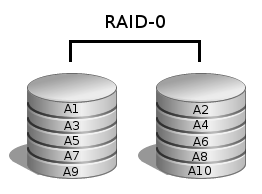
\includegraphics[width=.35\textwidth]{04/pics/raid-0}}
	\qquad
	\subfloat[Mirroring]{\label{fig:file-systems:raid-1}
			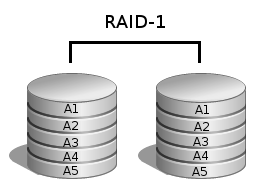
\includegraphics[width=.35\textwidth]{04/pics/raid-1}} \\
	\subfloat[Block-level striping with distributed parity]{\label{fig:file-systems:raid-5}
			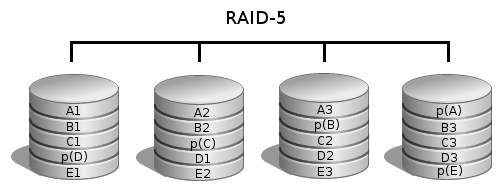
\includegraphics[width=.7\textwidth]{04/pics/raid-5}}
	\caption[RAID Levels illustrated]{Three of the most common RAID
		levels illustrated. RAID 0 increases performance, as blocks are
		written in parallel across all available disks. 
		RAID 1 provides redundancy, as blocks are written
		identically to all available disks.  RAID 5 aims to
		provide increased disk space as well as redundancy,
		as data is striped and parity information distributed
		across all disks.
		\label{fig:file-systems:raid}}
\end{figure}


\subsubsection{RAID 5}
\index{RAID!Level 5}

This level provides a bit of both RAID 0 and RAID 1:
data is written across all available disks, and for
each such stripe the data parity is recorded.  Unlike
in levels 2 through 4, this parity is not stored on a
single, dedicated parity drive, but instead
distributed across all disks.  See Figure
\ref{fig:file-systems:raid-5} for an illustration of
the block distribution.

Since parity information is written in addition to the
raw data, a RAID 5 cannot increase disk capacity as
linearly as a RAID 0.  However, any one of the drives
in this array can fail without impacting data
availability.  Again, as in the case of a RAID 1
configuration, the array will go into {\em degraded}
mode and get rebuilt when the failed disk has been
replaced.  However, the performance of the array is
decreased while a failed drive remains in the array,
as missing data has to be calculated from the parity;
the performance is similarly reduced as the array is
being rebuilt. Depending on the size of the disks
inquestion, this task can take hours; all the while
the array remains in degraded mode and another failed
drive would lead to data loss.

\subsubsection{Composite RAID and Failure Rates}

Since a RAID configuration creates a (virtual) disk to
present to the upper layer (such as the OS), it should
not come as a surprise that it is possible to combine
or nest RAID levels to achieve a combination of the
benefits provided by either one level; Table
\ref{table:file systems:raid-nested} lists some of the
most popular combinations.  In each case, we increase
fault tolerance at the expense of efficiency.

\begin{table}[b]
\centering
	\begin{tabular}{ l p{.75\textwidth}}
	\hline
	{\bf RAID 0+1} & Mirrored array of stripes \\
	{\bf RAID 1+0} & Striped array of mirrors \\
	{\bf RAID 5+0} & Striped array of multiple RAID 5 \\
	\hline
	\end{tabular}
	\caption{Standard RAID levels can be combined.}
	\label{table:file systems:raid-nested}
\end{table}

It is worth noting that the redundancy gained by
combining RAID levels is frequently overestimated.
Here's why: each drive has an expected failure rate,
each array a mean time to data loss.  The
``Independent'' in RAID misleads us to believe that
the odds of any one disk failing is entirely unrelated
to the others.  In reality, it is most common to use
identical drives from the same manufacturer if not
even the same production batch in a given array.  That
is, when a single drive fails and the array goes into
degraded mode, the probability of a second drive
failing is actually higher than one would expect with
truly independent drives.

Secondly, the actions performed by the RAID on the
disks needs to be taken into consideration as well.
When a disk in a RAID 5 array fails and is replaced,
{\em all} of the disks will undergo additional stress
as {\em all} of the data is read in order to rebuild
the redundant array.  This process may well take
several hours if not days -- a very long period of
time during which our data is at increased risk.  In
other words, the failure of a single drive will
necessarily increase the probability of failure of the
other drives\footnote{RAID 6 improves this situation,
at the expense of efficiency.  Dropping prices have
not very surprisingly lead more and more enterprise
environments to consider this trade-off entirely
acceptable.}.

When choosing a composite RAID architecture, it is
well worth our time to consider the Mean Time to
Recovery\index{Mean Time to Recovery} (MTTR) in
addition to the other factors.  From the moment that
a disk failure is detected until the array has been
rebuilt, our data is at severe risk.  In order to
reduce the MTTR, many system administrators deploy
so-called {\em hot spares}\index{hot
swapping}\index{RAID!Hot Spare}, disks that are
installed in the server and known to the RAID
controller, but that are inactive until a disk failure
is detected.  At that time, the array is immediately
rebuilt using this stand-by drive; when the faulty
disk has been replaced, the array is already in
non-degraded mode and the new disk becomes the hot
spare.

\begin{figure}[ht]
	\centering
	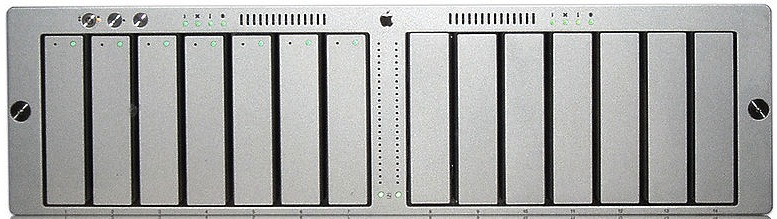
\includegraphics[width=.75\textwidth]{04/pics/xraid}
		\caption[Apple Xserve RAID]{An Apple Xserve RAID, a
			now discontinued storage device with 14 Ultra-ATA
			slots offering Fibre Channel connectivity and
			implementing a number of RAID levels in hardware
			as well as software across two independent
			controllers.
			\label{fig:file-systems:xraid}}
\end{figure}

\begin{figure}
\begin{experience}
{\bf Spectacular File System Confusion} \\

In early 2006, while working at Stevens Institute of
Technology as a System Administrator, we bought a new
Apple Xserve RAID storage device (like the one seen in
Figure \ref{fig:file-systems:xraid}) and populated its
14 disk slots with 400 GB drives, yielding (after
RAID, file system overhead and the previously
discussed discrepancy in binary versus decimal units)
two RAID5 configurations with a capacity of 2.2 TB
each, an impressive amount of affordable storage space
at the time. \\ [10pt]

The ``left'' RAID was dedicated to storing large
amounts of video and audio data made available to
clients running Mac OS X.  We connected the RAID
controller via Fibre Channel to a SAN switch, and from
there to an Apple Xserve network server, which managed
the HFS+ file system on this storage component. \\
[10pt]

The second 2.2 TB of storage space, the ''right'' side
of the array, was meant to become the central data
space for all workstations in the Computer Science and
Mathematics departments as well as their laboratories.
Up until then, this file space had been provided via
NFS from a two-module SGI Origin 200 server running
IRIX\index{IRIX}, managing a few internal SCSI disks as well
as some Fibre Channel direct attached storage.  We
intended to migrate the data onto the XServe RAID, and
to have it served via a Solaris 10 server, allowing us
to take advantage of several advanced features in the
fairly new ZFS and to retire the aging IRIX box.  \\
[10pt]

Neatly racked, I connected the second RAID controller
and the new Solaris server to the SAN switch, and then
proceeded to create a new ZFS file system.  I
connected the Fibre Channel storage from the IRIX
server and started to copy the data onto the new ZFS
file system.  As I was sitting in the server room, I
was able to see the XServe RAID; I noticed the lights
on the {\em left} side of the array indicate
significant disk activity, but I initially dismissed
this as not out of the ordinary.  But a few seconds
later, when the right side still did not show any I/O,
it dawned on me: the Solaris host was writing data
over the live file system instead of onto the new
disks!
\end{experience}
\end{figure}
% XXX remove pic?
\begin{figure}
\begin{experience}
\ContinuedFloat
I immediately stopped the data transfer and even
physically disconnected the Solaris server, but the
damage was done: I had inadvertently created a new ZFS
file system on the disks already containing (and
using) an HFS+ file system!  As it turns out, I had
not placed the Solaris server into the correct SAN
zone on the Fibre Channel switch, meaning the only
storage device it could see was the left side of the
array.  But since both sides of the array were
identical (in size, RAID type, manufacturer), it was
easy for me not to notice and proceed thinking that
due to proper SAN zoning, it was safe for me to write
to the device. \\ [10pt]

Now it was interesting to note that at the same time
as I was overwriting the live file system, data was
still being written to and read from the HFS+ file
system on the Apple server.  I was only able to
observe intermittent I/O errors.  Thinking I could
still save the data, I made my next big mistake: I
shut down the Apple server, hoping a clean boot and
file system check could correct what I still thought
was a minor problem.  \\ [10pt]

Unfortunately, however, when the server came back up,
it was unable to find a file system on the attached
RAID array!  It simply could not identify the device.
In retrospect, this is no surprise: the Solaris server
had constructed a new (and different) file system on
the device and destroyed all the HFS+ specific file
system meta data stored at the beginning of the disks.
That is, even though the blocks containing the data
were likely not over written, there was no way to
identify them.  After many hours of trying to recreate
the HFS+ meta data, I had to face the fact this was
simply impossible.  What was worse, I had neglected to
verify that backups for the server were done before
putting it into production use -- fatal mistake number
three!  The data was irrevocably lost; the only plus
side was that I had learned a lot about data recovery,
SAN zoning, ZFS, HFS+ and file systems in general.

\end{experience}
\end{figure}

\section{File Systems}
\label{sec:file systems}
\index{File Systems}

When the operating system is installed, it will create
a file system on the specified disk(s).  As we have
seen, these disks may be made available to the OS in a
variety of ways, but in the end, the OS does not
distinguish between a \gls{das} device such as a hard drive
disk, a volume created by an \gls{lvm}, a disk represented
by a RAID or one backed by a storage device over a
SAN.  This method of hiding hardware implementation
choices or details allows the OS to choose amongst a
number of different file systems, each with their own
unique strengths, disadvantages and performance
impacting tuning options.

Reduced to its most basic tasks, a file system is
responsible for storing, managing and updating data on
the storage device in question.  To this end, it needs
to manage the available space and be able to store
files as well as their attributes (i.e. {\em
metadata}) in a hierarchy that allows both the user
and the OS to efficiently retrieve them, as well as
ensure some level of file and file system integrity.
In addition, since Unix is a multi-user OS, the file
system depends on means to identify and distinguish
between different users; access control and the
concepts of {\em file permissions} are a basic
requirement.  What's more, Unix systems frequently
represent as ``files'' many things that us humans may
not usually think of as such\footnote{The ``Plan 9
from Bell Labs\index{Bell Laboratories}'' research
operating system\index{Plan 9} took the initial Unix
mantra of ``everything is a file'' much further: all
objects are either files or file systems,
communicating with each other via the {\em 9P}
protocol.  Network connections, communications with
the kernel's drivers, interprocess communication etc.
all are performed via standard I/O calls.}.  This
leads us to special purpose file systems that really
only provide a file I/O \gls{api} to their respective
resources: the {\em procfs}\index{procfs} file system,
representing information about the system's processes
and the {\em devfs}\index{devfs} file system, a
virtual file system acting as an interface to device
drivers are two examples.

\subsection{File System Types}
\label{file systems:types}

In this section, we will take a look at some of the
file systems commonly in use on Unix systems.  For the
most part, these are {\em disk file systems}, meaning
that they are designed to manage hard disk storage.
As we've seen in previous sections, the physical
layout of a hard drive influences partitioning
schemas, but the choice and creation of the operating
system's file system may also depend on the underlying
hardware.

As we discuss these file systems, we will find that
the approach to store both the actual file data as
well as the metadata, the information associated {\em
with} the files, differs significantly.  We will also
notice -- as a recurring pattern throughout this book
-- how different layers of abstraction help us improve
portability and provide a consistent interface, as
standard file I/O semantics can remain the same across
different file systems.

\subsubsection{Disk File Systems}
\index{File Systems!Disk}

A {\em Disk File System} is probably what most people
-- at least those who {\em would} think about these
kinds of things to begin with -- have in mind when they
think about what a file system does.  It manages block
device storage, stores ``files'' in ``directories'',
maintains a file system hierarchy, controls file
metadata, and allows for simple I/O via a few basic
system calls.  The canonical file system for the Unix
family of operating systems is, of course, the {\em
Unix File System} (\gls{ufs})\index{File Systems!UFS},
also known as the {\em Berkeley Fast File System}
(\gls{ffs})\index{Fast File System}.  We will look at
the UFS in detail in Section
\ref{sec:unix-file-system}, but for now suffice it to
say that this file system implementation and its use
of boot blocks, superblocks, cylinder groups,
{\em inodes}\index{inode} and data blocks is repeated and
reflected in many other Unix file systems, including
for example {\em ext2}\index{File Systems!ext2}, for a
long time the default file system for Linux systems.

These traditional file systems suffer a notable
drawback in the case of unexpected power failure or a
system crash: some of the data may not have been
committed to the disk yet, causing a file system
inconsistency.  When the OS boots up again, it will
need to perform time consuming checks (see
\manpage{fsck(8)}) and any problems found may not
actually be recoverable, leading to possible data
loss.  In order to address these problems, a so-called
{\em journaled} file system might choose to first
write the changes it is about to make to a specific
location (the journal) before applying them.  In the
event of a crash, the system can then simply replay
the journal, yielding a consistent file system in a
fraction of the time it would take a traditional file
system to traverse the entire hierarchy to ensure
consistency.

There are many different journaled file systems,
including a number of commercial implementations (such
as Apple's {\em HFS+}\index{File Systems!HFS+}, IBM's
{\em JFS}\index{File Systems!JFS}, or SGI's {\em
XFS}\index{File Systems!XFS}) and open source variants
(including {\em ext3}, {\em ext4}\index{File
Systems!ext3}\index{File Systems!ext4} and {\em
reiserfs}\index{File Systems!reiserfs} for Linux and
updates to UFS/FFS providing support for journaling or
logging).

Despite the differences in how data is ultimately
written to the disk, the fundamental concepts of how
data and metadata are managed, the use of the {\em
inode} structures, or the {\em Virtual File System}
layer to allow the kernel to support multiple
different file systems remains largely the same across
the different Unix operating and file systems.

\subsubsection{Distributed File Systems}
\index{File Systems!Distributed}

Unlike a disk file system, which provides access to
the data it holds only to the processes running in the
operating system the disk is attached to, a {\em
distributed file system} may allow different client
systems to access a centralized storage resource
simultaneously, thus forming the basis for any
\gls{nas} solutions.  As we discussed in Section
\ref{file systems:storage-models:nas}, this model
implies that clients no longer operate on the block
level of the storage -- this access has been
abstracted on a higher level and the client OS thus
requires in-kernel support for the file system in
question.

Sun Microsystems\index{Sun Microsystems}' {\em Network
File System} (\gls{nfs})\index{File Systems!NFS},
created in 1985, was the first such file system
utilizing the {\em Remote Procedure
Calls}\index{Remote Procedure Calls} (RPC) via the
Internet Protocol (IP)\glslink{ip}\index{Internet
Protocol} for the server to communicate with the
clients, and remains to this day the standard
distributed file system in the Unix world.  Other
notable variations include the {\em Andrew File
System} (\glslink{afs}{AFS})\index{File Systems!Andrew
File System/AFS} and its descendent, {\em Coda},
developed at Carnegie Mellon University\index{Carnegie
Mellon University}, tightly integrated with the
Kerberos\index{Kerberos} authentication protocol, and
backed by a local cache, making it particularly
tolerant of network interruptions, as well as the {\em
Server Message Block}/{\em Common Internet File
System} ({\em
\glslink{smb}{SMB}/\glslink{cifs}{CIFS}}), the
predominant network file system in the Windows world,
made accessible to Unix systems via the
``Samba''\index{Samba} implementation of these
protocols.

Within the area of massive scale Internet systems, a
number of specialized, distributed file systems have
emerged, most notably the {\em Google File
System}\cite{filesystems:gfs}\index{File
Systems!Google/GFS} and the {\em Hadoop Distributed
File System}\cite{filesystems:hdfs}\index{File
Systems!Hadoop/HDFS} (the latter being an open source
implementation modeled after the former).  These file
systems provide highly scalable fault tolerance while
at the same time providing high performance on
low-cost commodity hardware.

As usual, different problems call for different
solutions, and despite their significant capabilities,
these file systems may not necessarily be suitable for
your requirements.  In fact, making use of these
capabilities requires a significant investment -- both
in the time and expertise required to manage them as
well as in the hardware required to really get
anything out of them.

Other distributed file systems may have a different
focus, leading to interesting and entirely distinct
properties: the {\em Tahoe Least-Authority File
System}\cite{filesystems:tahoe-lafs}\index{File
Systems!Tahoe Least-Authority}, for example, provides
data confidentiality through the use of cryptography,
thus allowing complete decentralization over the
(public) Internet.  On the other hand, the advent of
cloud computing has further blurred the boundaries of
where a distributed file system ends and where a
network service begins: Amazon's {\em Simple Storage
Service} (\glslink{s3}{S3})\index{AWS!S3}, for
example, despite being an \gls{api} driven web
service, might as well be considered a distributed
file system, but then so could online storage
providers, such as Dropbox, who build their
solutions on top of Amazon's service.  It will be
interesting to see how these distributed file systems
or data stores evolve with time.


\subsubsection{``Other'' File Systems}
\index{File Systems!Special Purpose}

In the Unix world, there exists an old mantra:
``Everything is a file.'' That is, the simple
\gls{api} defining file I/O has proven so useful that
a number of non-file ``things'' have come to implement
this interface as well: not only can regular files be
accessed using the \manpage{open(2)},
\manpage{read(2)}, \manpage{ write(2)} and
\manpage{close(2)} system calls\footnote{All of these
system calls operate on a small non-negative integer,
the so-called file {\em descriptor} or file {\em
handle}.  The old expression should therefore more
accurately be cited as ``Everything is a file
descriptor.''}, but so can network sockets and other
interprocess communication endpoints, character and
block devices, so-called {\em pseudo-devices} (such as
{\tt /dev/null}\index{\tt /dev/null}), and various
other ``special files''.

Similarly, a number of pseudo- and virtual file
systems have been created to use the same \gls{api}
and make resources available using file-like
structures.  The access points for these structures
becomes a mount point in the file system hierarchy,
{\em et voil\`{a}}, these resources can be accessed,
processed and manipulated using common Unix tools.
Examples include the {\em devfs}\index{File
Systems!Device} virtual file system (used to access
special and general devices), the {\em procfs} pseudo
file system (providing information about system
information and individual processes), the {\em
UnionFS}\index{File Systems!Union} (a method of
layering two regular file systems on top of each
other, providing the union of the two hierarchies to
the user), and {\em tmpfs}\index{File
Systems!Temporary} (a method of creating a file system
in virtual memory, granting significant performance
benefits).

In addition to these cases, there are also a number of
file systems that have been created to meet very
specific requirements, or that effectively function as
an overlay on top of an application or protocol in
order to facilitate local file access to remote
resources, such as, for example, the SSH file system.
But file systems are usually implemented in the
operating system's kernel space: file I/O system calls
do happen here and devices and certain other resources
can only be controlled by the kernel; likewise,
mounting or unmounting file systems requires superuser
privileges.  But not all file systems are actually
accessing any of the resources protected by the
kernel.  In order to facilitate non-privileged access
to file system interfaces, some Unix systems have
created kernel modules that provide a method to
implement virtual ``File Systems in
Userspace''\index{File Systems!Userspace/Fuse} (known
as {\em FUSE}).

All of these file systems that aren't actually {\em
file} systems but rather an abstraction of other
resources into a file \gls{api} illustrate how much the
concept of simplicity permeates the Unix culture.  At
this point, few system administrators would wish to
part with the convenience of, for example, {\em
procfs} -- in fact, its availability is almost
universally assumed.  For a polyglot administrator,
however, it is important to be familiar with the
different pseudo- and virtual file systems available
on the different Unix versions and, more importantly,
know how to access the resources they represent in
their absence.

\section{File System Layout}
\label{file systems:layout}

The traditional Unix file system layout is organized
as a tree-like hierarchy, rooted at {\tt /}
(``slash'').  Under this directory reside a number of
standard top-level subdirectories, each with a
well-defined purpose and containing further
subdirectories, forming a hierarchy described in the
{\tt hier(7)}\index{\tt hier(7)} manual page.

Unix systems can make use of multiple different file
systems on multiple partitions at the same time.  Each
may be attached or ``mounted'' under any directory (or
``mount point'') of the file system hierarchy with the
exception of the root file system: the file system
containing the basic operating system and from which
the system was booted, which must be mounted at {\tt
/}.

Figure \ref{fig:file-systems:layout} illustrates a
subtree of the typical Unix hierarchy with different
components residing on separate disks.  Each node in
the tree represents a directory entry used to map
file names to inodes\index{inode}; nodes with children
represent directories, leaf nodes represent regular
files.  Traversing the tree from the root to any given
node constructs a so-called
``pathname\index{pathname}'' consisting of directory
names concatenated with a path separator, ``{\tt /}'',
followed by the file name.

\begin{figure}[ht]
	\centering
	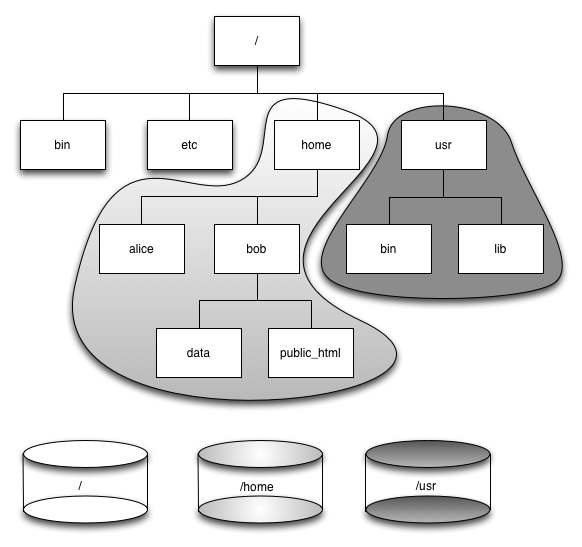
\includegraphics[width=.75\textwidth]{04/pics/filesystem-tree-mountpoints}
		\caption[File System Hierarchy]{The Unix file system is a
			tree-like structure, rooted at {\tt /}; 
			different file systems can be attached at
			different directories or mount points.  In
                        this illustration, {\tt /home} and {\tt /usr}
                        reside on separate disks from {\tt /}.
			\label{fig:file-systems:layout}}
\end{figure}


File names may contain any character except for this
separator or the {\em NUL} character ({\tt
\textbackslash0}), used in the the C programming
language to terminate a string.\footnote{It is a
common mistake to assume that a file name contains
only printable characters.  The Unix system does not
impose many restrictions on how a user might choose
to name a file, and file names containing e.g. control
characters such as a carriage return (``{\tt \\n}''),
while confusing on a line-buffered terminal, are
possible.}  Most Unix systems impose a maximum file
name length of 255 bytes and a maximum pathname length
of 1024 bytes; however, these are file system and OS
specific limits.

Every Unix process has the concept of a current
working directory -- run the \manpage{pwd(1)} command
or type ``{\tt echo \$PWD}'' in your shell to display
where in the file system hierarchy you currently are.
Pathnames may either be {\em relative} to this
location, or, if they begin with a {\tt /}, {\em
absolute}.

Each directory contains at least two entries: ``{\tt
.}'' (dot), a name for the current working directory
and ``{\tt ..}'' (dot-dot), a name for the parent
directory.\footnote{As a special case, within the root
directory both ``{\tt .}'' and ``{\tt ..}'' refer to
the same directory, i.e. {\tt /}.}  Since relative
pathnames are resolved from within the current working
directory, the same file can be referred to by
different names, as shown in the examples in Listing
\ref{code:pwd}.

\begin{lstlisting}[float,basicstyle=\scriptsize,label=code:pwd,caption={[Absolute
and relative pathnames] Absolute pathnames begin with
a {\tt /} and are resolved from the root of the file
system; relative pathnames are resolved from the
current working directory.}]
$ pwd
/home/jschauma              # pwd(1) writes the absolute pathname
$ echo hello > file         # create "file" in the current directory
$ cd /usr/share/doc         # cd(1) using an absolute pathname
$ pwd
/usr/share/doc              # no surprise here
$ cat /home/jschauma/file   # now using an absolute pathname
hello
$ cd ../../../home/jschauma # cd(1) using a relative pathname
$ pwd
/home/jschauma
$ cat file                  # "./file" would also work
hello
$ 
\end{lstlisting}

\section{The Unix File System}
\label{sec:unix-file-system}
\index{File Systems!Unix}\index{Unix File System}\index{UFS}\index{FFS}

As we discuss the general concepts of file systems in
the Unix world, it is impossible to avoid a much
closer look at the {\em \acrlong{ufs}} (\gls{ufs}),
the initial standard file system for a
number of both commercial and open source Unix
versions for decades.  UFS, also known as the {\em
Berkeley Fast File System} or \gls{ffs}, created by
Marshall Kirk
McKusick\cite{filesystems:ffs}\index[names]{McKusick,
Marshall Kirk} and others at the University of
California in Berkeley in 1984, was a reimplementation
of the original file system provided by Bell
Lab\index{Bell Laboratories}'s UNIX\index{UNIX} V7.

\begin{figure}[t]
	\centering
	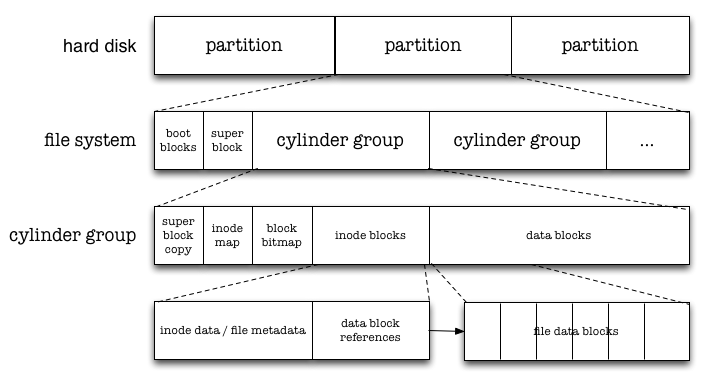
\includegraphics[width=.85\textwidth]{04/pics/ufs-details}
		\caption[UFS Details]{A disk may be divided into multiple
			partitions; a partition may contain a file system
			with multiple cylinder groups; each cylinder group
			contains some file system meta data as well as
			inode and data blocks.
			\label{fig:file-systems:ufs-details}}
\end{figure}

These improvements and changes introduced most notably
the concept of cylinder groups, providing a more equal
distribution of the file metadata on the physical
disk, thus minimizing seek time.  The Unix File System
therefore consisted of the following major components,
as illustrated in Figure
\ref{fig:file-systems:ufs-details}:

\begin{itemize}
	\item A {\bf superblock}\index{superblock}.  This block contains all the
		system's crucial information, such as the number and
		location of cylinder groups used as well as the location of the
		inode and data blocks.  As this information is critical for
		the operation of the file system and corruption of this
		block would be disastrous, it is replicated and stored in
		a number of (predictable) locations.  This allows
		the super user to repair a corrupted file system by pointing to an
		alternate superblock.
	\item A number of {\bf cylinder groups}\index{cylinder groups}, which break the large
		file system into more manageable chunks by distributing
		meta data evenly across the physical partition.
	\item A number of {\bf inode maps} (one for every cylinder group),
		pointing to the cylinder group's {\bf inode blocks}, which
		in turn contain the metadata associated with the files.
	\item A number of {\bf block bitmaps} (one for every cylinder
		group), pointing to the cylinder group's {\bf data blocks},
		which in turn contain the actual file data.
\end{itemize}

The distribution of this data across multiple cylinder
groups illustrates the tight relationship that the
file system had with the physical properties of a hard
disk drive; this layout remains in place nowadays,
even though on solid state drives, for example, we no
longer suffer performance penalties due to seek time.

It is important to note that the data blocks used by
the file system are different from the {\em physical}
blocks of the hard disk.  The latter are, as we
discussed in Section
\ref{sec:file-systems:physical-disk-structure}, 512
bytes in size (or, in more recent drives, 4096 bytes);
the former -- called the {\em logical} block size --
can be decided on by the system administrator at file
system creation time.  UFS uses a minimum logical
block size of 4096 bytes, and defaults to larger block
sizes based on the overall size of the file system.
Likewise, the number of inodes in a file system is
fixed once the file system has been created.  Here,
UFS defaults to an {\em inode density} of one inode
per 2048 bytes of space for small file systems --
consult the \manpage{newfs(8)} manual
page for this and other parameters to define and tune
the file system at its creation time. \\


Let us dive a little bit deeper and think about how
the Unix File System manages disk space:  A file
system's primary task is to store data on behalf of
the users.  In order to read or write this data, it
needs to know in which logical blocks it is located.
That is, the file system needs a map of the blocks, a
way to identify and address each location.  This is
accomplished by way of the {\em inode} and {\em data
block} maps: the total number of inodes represents the
total number of files that can be referenced on this file
system, while the data blocks represent the space in
which the file data is stored.

As we noted, a data block is, necessarily, of a fixed
size.  That means that if we wish to store a file that
is larger than a single block, we have to allocate
multiple blocks and make a note of which blocks
belong to the given file.  This information is stored
as pointers to the disk blocks within the
inode\index{inode} data structure.

Unfortunately, however, not all files will be
multiples of the logical block size.  Likewise, it is
possible that files will be smaller than a single
block.  In other words, we will always end up with
blocks that are only partially allocated, a waste of
disk space.  In order to allow more efficient
management of small files, UFS allowed a logical block
to be divided further into so-called {\em fragments},
providing for a way to let the file system address
smaller units of storage.  The smallest possible
fragment size then is the physical block size of the
disk, and logical blocks are only fragmented when
needed.

A pointer to the data blocks and fragments allocated
to a given file is stored in the inode data structure,
which comprises all additional information about the
file.  This allows for an elegant separation of a
file's metadata, which takes up only a fixed and small
amount of disk space, and its contents.  Accessing the
metadata is therefore independent of the file size
(itself a piece of metadata), allowing for efficient
and fast retrieval of the file's properties without
requiring access of the disk blocks.  Other pieces of
information stored in the inode data structure include
the file's permissions, the numeric user-id of the
owner, the numeric group-id of the owner, the file's
last access, modification and file status change
times\footnote{A file's {\tt ctime}, it's time of last
file status change, is frequently misinterpreted to be
the file's {\em creation} time; most file systems,
including UFS, do {\em not} store this kind of
information.  Instead, the {\tt ctime} reflects the
last time the meta information of a file was
changed.}, the number of blocks allocated for the
file, the block size of the file system and the device
the file resides on, and of course the inode number
identifying the data structure.

% XXX: formatting/wrapping?
\begin{lstlisting}[float,basicstyle=\scriptsize,label=code:ls-ai,caption={[Output
of {\tt ls -ai}]Use of the ls(1) command on a NetBSD
system to illustrate how file names are mapped to
inode numbers in a directory.  (Note that in the root
directory both '.' and '..' have the same inode
number\, as in this special case they actually are the
same directory.)}]

$ ls -ai /
      2 .         5740416 cdrom    5816448 libexec  2775168 stand
      2 ..        1558656 dev      1862784 mnt      2166912 tmp
3003280 .cshrc     988439 emul           4 netbsd   3573504 usr
3003284 .profile   342144 etc      1824768 proc     3497472 var
3421440 altroot   1026432 home      798336 rescue
5702400 bin       3763584 lib      3003264 root
      3 boot.cfg  2204928 libdata  5588352 sbin
$
\end{lstlisting}

Now humans tend to be rather bad at remembering large
numbers and prefer the use of strings to represent a
file, but the one piece of information that is {\em
not} stored in the inode is the file name.  Instead,
the Unix File System allows for a mapping between a
file name and its unique identifier -- its inode --
through the use of directories.  A directory really is
nothing but a special type of file: it has the same
properties as any other file, but the data it holds is
well-structured (in contrast to the byte stream
contained in so-called ``regular'' files) and consists
of inode number and file name pairs.  You can use the
\manpage{ls(1)} command to illustrate this --
see Listing \ref{code:ls-ai}.

A mapping of an inode number to a file name is called
a {\em hardlink}\index{link!hard}, even though humans
tend to prefer the term ``file name''. An inode can be
accessed by more than just one file name: within a
single file system, each file may be referenced by
multiple names in different directories, and the
number of hardlinks for a given file is stored in the
inode data structure as well.  But since each file is
identified by its inode number, and since multiple
file systems can be mounted in a running operating
system, it is possible that two files on two different
file systems have the same inode number.  As a result,
a file is really only uniquely identified by its
combination of file system device and inode number.
What's more, at times it may be useful to create a
pointer to a file residing on a different file system,
but as just explained, creating a hard link across
file system boundaries is impossible.  To overcome
this limitation, so-called ``symbolic
links''\index{link!symbolic} were invented: a symbolic
link (often abbreviated as ``symlink'') is a special
kind of file that contains as its only contents the
path name of the file it references.  Almost all
operations on a symlink will then be redirected to the
target file it points to.

In addition to regular files (hard links), directories
and symbolic links, the following file types are
supported by the traditional Unix file system:

\begin{itemize}
	\item {\em Block special devices} -- an interface for disk-like
		devices, providing buffered and non-sequential I/O.
	\item {\em Character special devices} -- an interface for
		communication devices such as keyboards, mice, modems, or
		terminals, providing unbuffered I/O.  A number of virtual,
		so-called pseudo-devices such as {\tt /dev/null}\index{\tt /dev/null}, {\tt
		/dev/zero}\index{\tt /dev/zero},  or {\tt /dev/urandom}\index{\tt /dev/urandom}, for
		example, are also accessed as character special devices.
	\item Named pipes or {\em FIFO}s -- another inter-process
		communications endpoint\index{IPC!FIFO} in the file
		system.  This type of file represents a manifestation of
		the traditional Unix pipe in the file system name space;
		I/O is performed using the same methods as for any regular
		file.  As data is merely passed between processes, a FIFO
		always has a file size of zero bytes.
	\item Unix domain {\em sockets} -- an inter-process communications
		endpoint\index{IPC!Unix domain socket} in the file system
		allowing multiple processes with no shared ancestor
		process to exchange information.  Communication happens
		via the same \gls{api} as is used for network sockets.
\end{itemize}

\begin{lstlisting}[float,label=code:stat,caption={[Output of {\tt stat(1)}]Sample
output of the stat(1) command on a Linux system\, showing the various pieces of
information stored in the inode data structure for the file ``/etc/passwd''.}]
$ stat /etc/passwd
  File: `/etc/passwd'
  Size: 2062      	Blocks: 8       IO Block: 4096   regular file
Device: ca02h/51714d	Inode: 725181   Links: 1
Access: (0644/-rw-r--r--)  Uid: (0/root)   Gid: (0/root)
Access: 2011-08-26 23:45:31.000000000 -0400
Modify: 2011-08-26 23:45:31.000000000 -0400
Change: 2011-08-26 23:45:31.000000000 -0400
$
\end{lstlisting}

The file type as well as its permissions and all the
other properties of a file can be inspected using the
\manpage{stat(1)} command (see Listing \ref{code:stat}
for an example), or, perhaps more commonly, using the
\manpage{ls(1)} command (as illustrated in Figure
\ref{fig:file-systems:ls-l}).  This command is so
frequently used and its output so ubiquitous that any
system administrator can recite the meaning of the
fields in their sleep.  The semantics and order in
which permissions are applied, however, include a few
non-obvious caveats, which is why we will look at the
Unix permissions model in more detail in Chapter
\ref{chap:multi-user}. \\

Over the last 30 years, UFS has served as the
canonical file system for almost all Unix versions.
With time, a number of changes have become necessary:
more fine-grained access controls than the traditional
Unix permissions model allows were made possible via
file system extensions such as
\gls{acl}s\index{Access Control Lists}; larger storage
devices required not only updates to the block
addressing schemas, but also to the different data
types representing various file system aspects;
today's huge amounts of available data storage have
made log-based file systems or journaling capabilities
a necessity, and massively distributed data stores
pose entirely different requirements on the underlying
implementation of how the space is managed.

Yet through all this, as enhancements have been made
both by commercial vendors as well as by various open
source projects, the principles, the very fundamentals
of the Unix File System have remained the same:  the
general concept of the inode data structure and the
separation of file metadata from the data blocks have
proven reliable and elegant in their simplicity.  At
the same time, this simplicity has proven to yield
scalability and adaptability: the persistent idea that
``everything is a file'', and that files simply
store bytes and thus have no inherent structure
(unlike a database or certain archives) have allowed a
surprising flexibility and lead to the creation of
many pseudo- or virtual file systems providing a
simple \gls{api} and User Interface (UI) to any number
of resources.

\begin{figure}[t]
	\centering
	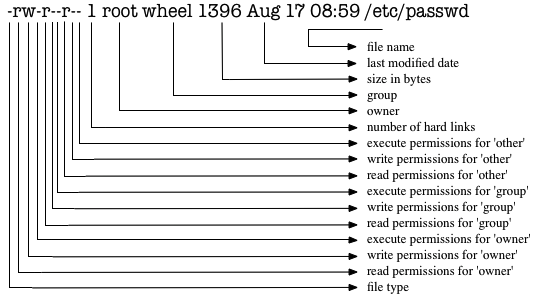
\includegraphics[width=.75\textwidth]{04/pics/ls-l}
		\caption[File Metadata]{The default output of the {\tt ls -l}
			command includes most of the metadata of a given
			file.
			\label{fig:file-systems:ls-l}}
\end{figure}

\section{Conclusions}
\label{file systems:conclusions}

Throughout this chapter, we have built our
understanding of file systems and storage models from
the ground up.  We have seen how simple concepts are
combined to construct increasingly complex systems --
a pattern that weaves like a red thread through all
areas we cover.  We noted the circular nature of
technology development: the simple \gls{das} model
repeats itself, albeit more complex and with
additional layers, in common SANs, much as network
attached storage utilizes both DAS and SAN solutions,
yet is taken to another extreme in cloud storage
solutions.

Being aware of the physical disk structure helps us
understand a file system's structure: we realize, for
example, that concentric cylinder groups make up
partitions, and that the location of data blocks
within these cylinders may have an impact on I/O
performance.  What's more, the concepts of file system
blocks become clearer the further we deepen our
knowledge of both the logical and physical components,
and the distinction of metadata from the actual
contents of a file allow us to explain how the various
file system related Unix tools operate on a fairly low
level as well as how to tune these values at file
system creation time.  As system administrators, this
understanding is crucial.

But what about our earlier point of noting the three
pillars of strong system architecture and design:
Scalability, Security, Simplicity.  What role do these
play in the context of file systems and storage
models? \\

Scalability is defined by our aptitude to meet
changing requirements.  As far as file systems are
concerned, we need to be able to provide sufficient
storage that meets our performance and rapidly
increasing space requirements.  One might be tempted
to jump to a quick conclusion and choose the
superficially ``most flexible'' solution, which
nowadays often appears to be a cloud based storage
model.  However, it behooves us to take a step back
and consider the other two major design decisions,
simplicity and security, which help us cut through
complexities and clarify just how flexible such a
model might be.  Reliance on a third party provider
for data storage, for example, incurs a number of
hidden costs: bandwidth requirements increase, data
redundancy and duplication need to be weighed, backup
and data migration strategies change radically, and
vendor lock-in may in fact eliminate true
flexibility.\footnote{Depending on the size of your
organization, these costs may in fact not be hidden
at all: at some point, you may find yourself providing
``cloud storage'' to your organization, and all of a
sudden you are the owner of that infrastructure.}.

So what makes for a scalable storage solution?  On the
one hand, we need to be able to add disk space on
demand, so we either require a file system that can
grow as needed, or an efficient way to synchronize
multiple file systems.  This already illustrates a
trade-off in complexity and the solutions depend in
part on our network architecture:  within a single
system, the use of an \gls{lvm} or a file system that
allows the pooling of multiple resources seems a good
choice, but how do you make that available to multiple
clients?  If you have hosts in distinct geographical
locations, connected only via the Internet (an
inherently untrustworthy network), how do you allow
for shared access?

The more you think about these requirements, the more
you will find yourself weighing conflicting
approaches.  You will go back and forth between the
simplest possible solution (for example, all hosts
write data only to direct attached storage) and the
more complex (shared storage available via a
distributed file system or a cloud architecture).  But
it becomes increasingly hard to define ``simple'', as
each solution requires considerations outside of the
initial problem domain: hosts writing to \gls{das} is
efficient, but data synchronization across all hosts
becomes increasingly complicated; a shared storage
pool available over the network solves that problem,
but incurs a high cost of complexity and dependency on
the supporting infrastructure.

What's more, the security aspects of the file system
and the features it provides are manifold:  as Unix
was designed from the beginning as a multi-user
operating system, the capabilities to distinguish
between different users were built into the system and
is reflected in the file permissions.  But file system
security goes beyond this basic level, especially when
we consider access over the network.  Every
distributed file system has to solve the problem of
deciding whether or not a remote system should be
granted access to a given resource, and how such a
system should authenticate.  The access models range
from simplistic (if you are on the local network, you
are granted access) to the more sophisticated (a
client has to present some sort of time-limited
authentication token to gain access).

But a system administrator's professional paranoia
dictates digging {\em even} deeper.  In the case of
distributed file systems, of storage area networks or
of remotely hosted, cloud-based storage solutions, we
not only have to consider how a remote client
authenticates and is granted access, but also who has
access to the bits and bytes in transit, or how to
protect our data's confidentiality should a remote
system be compromised.  Is transport security assumed,
or do we rely on secure network connections (for
example on the network layer via a VPN or
IPsec\index{IPsec} tunnels, or on the application
layer via \glslink{tls}\index{TLS} or
SSH\index{SSH}, to name but a few examples)?  Is data
stored ``in the cloud'' accessible to anybody with
access to the physical device (simple, but trust is
placed into the storage provider, often a third
party), or do we encrypt it (more secure, but also
more complex)?  Under what jurisdiction is the data
stored, and what data could be subpoenaed by which
authorities?\index{government access}  Would you even
be notified if access to your and your users' data was
granted to law enforcement\index{law enforcement}? \\

As we will see throughout this book, there never is a
single solution to all our problems.  We will
continually have to make trade-offs based on
assumptions and probabilities, usability
considerations and practical concerns.  There is no
silver bullet, no one solution, no unique, always
correct approach.  This is why it is so important for
a system administrator to be aware of {\em all} the
factors, and to ask the questions we've started to
suggest here at the end of this chapter.  Not
surprisingly, this line of questions quickly leads us
beyond the basic concepts of file systems and storage
models, but likewise often brings us full circle when
we have to consider higher level applications and
consider just how exactly they access data and what
kinds of assumptions and requirements they pose as to
availability, security and performance.  The topics
covered in this chapter are the foundation upon which
our systems are built.

\vfill
\pagebreak

\chapter*{Problems and Exercises}
\addcontentsline{toc}{chapter}{Problems and Exercises}
\section*{Problems}
\addcontentsline{toc}{section}{Problems}

\begin{enumerate}

\item
Identify the storage area model(s) predominantly used in your
environment(s).  What kind of problems with each do you frequently
encounter?  Would changing the storage model be a feasible solution to
these problems?  Why or why not?

\item
Research the implementation details of a popular cloud storage provider.
What storage solutions did they choose?  Can you identify all the
different models we discussed?

\item
Identify at least three distinct security concerns in each of the storage
models we discussed.  Outline in detail how an attacker might exploit such
weaknesses and how a System Adminstrator might prevent or counter each
attack.

\item
\label{prob:disks:hdds}
Ask your system administrators if they have any old or broken hard drives,
if possible from different manufacturers or with different capacities.
Open up the drives and identify the various components.  How many
read-write heads are there?  How many platters?  How do the different
models differ?

\item
\label{prob:disks:disklabel}
Compare the output of the \manpage{fdisk(8)} command on different operating
systems.  Divide a disk into a number of different partitions, then use
\manpage{disklabel(8)} to review the resulting label.  Identify all the
different partitions, verify their capacities and explain any
discrepancies or unexpected findings.

\item
Compare the various composite RAID levels and analyze their respective
fault tolerance and mean time to recovery in the case of one or more
failed disks.

\item
Assuming 500 GB disk drives, what is the total capacity of a RAID
configuration using 7 disks under RAID 0, RAID 1, RAID 5, RAID 6, RAID
0+1, RAID 1+0 and RAID 5+0?

\item
You want to create a RAID 5 using several multi-terabyte
drives.  Research and choose your preferred hardware,
paying particular attention to their {\em
Unrecoverable Read Error}\index{Unrecoverable Read
Error} rates (i.e. the mean time to failure, usually
expressed as number of bits read).  If the array is
filled to capacity with data, and one of the drives
failes and has to be replaced, how much data do you
end up reading when you rebuild the array?  What does
this say about the probability of an additional disk
failure while you're still in degraded mode?

\item
Identify the different file systems in use on the Unix
versions you have access to.  How many partitions are
there, where are they mounted, what mount options do
they use?  Were they chosen explicitly or do they
appear to be OS defaults?

\item
Identify all resources made available by the {\em procfs} system, both
about the system and about individual processes.  Suppose {\em procfs} was
not available, how would you go about finding out the same information?

\item
Identify the different devices found under {\tt /dev}.  What is the
difference between {\tt /dev/null} and {\tt /dev/zero}, between {\tt
/dev/random} and {\tt /dev/urandom}?

\item
Identify the file system limitations on a system you have access to.  What
is the maximum file system size?  What is the maximum file size?  What
characters may be used in a file name?  How many files can you create in a
single directory?

\item
Compare at least four different file systems with respect to their default
block size and inode density.  Consider both small (less than 1 GB in
size), ``normal'', and very large (more than 1 TB in size) partitions or
volumes.  How efficiently does each system manage this space?  Can you
specify different inode and block sizes to increase efficiency?

\item
Review the concepts of inode mappings to file names, hard links, and
symbolic links.

\begin{enumerate}

\item
Create a new file, then create a second hard link for this file.  Verify
that both files are completely identical by using {\tt ls(1)}, {\tt
stat(1)} and by appending data to one of the files and reading from the
other.

\item
Rename the original file and repeat -- what changed?  Why?

\item
Create a new file, then create a symbolic link for this file.  Verify that
both the original file and the symbolic link are unique by inspecting
their inode numbers.  Then append data to the file using the regular name
and confirm that reading from the symbolic link yields the same data.

\item
Rename the original file and repeat -- what changed?  Why?
\end{enumerate}

\item

Create a very large file.  Measure how long it takes
to rename the file within one directory using the {\tt
mv(1)} command.  Next, use {\tt mv(1)} to move the
file into a directory on a different file system or
partition.  What do you observe?  Explain the
difference.

\item
Experiment with the usability, resilience and
limitations of a system's root file system.

\begin{enumerate}

\item
Identify how much free disk space you have, then fill
it up.  Can you use up all available space using a
single file?  What are the effects of using up all
disk space?  Can you still create new, empty files?
Can you still log in?  Why/why not?

\item
Identify how many free inodes are available on your
root file system, then use them up by, e.g., creating
lots and lots of empty files.  What happens to the
directory size in which you create these files?  What
is the error message once you run out of inodes?  Can
you still create new files?  Can you still write to
existing files?  How much disk space is available now?
Can you still log in?  Why/why not?

\end{enumerate}


\end{enumerate}

\pagebreak

\bibliographystyle{plainnat}
\begin{thebibliography}{99}

\bibitem{disks:emc2-storage} EMC Education Service,
{\em Information Storage and Management: Storing, Managing, and Protecting
Digital Information}, John Wiley \& Sons, 2009

\bibitem{disks:frisch} \AE leen Frisch, {\em Essential System
Administration}, O'Reilly Media, 2002

\bibitem{filesystems:gfs} Sanjay Ghemawat, Howard Gobioff, and Shun-Tak
Leung, {\em The Google File System}, in ``Proceedings of the nineteenth
ACM symposium on Operating systems principles'', 2003, ACM, New York, NY;
also available on the Internet at
{\url http://research.google.com/archive/gfs-sosp2003.pdf}
(visited September 6th, 2012)

\bibitem{filesystems:hdfs} {\em The Hadoop Distributed File System:
Architecture and Design}, on the Internet at
{\url https://hadoop.apache.org/common/docs/r0.14.4/hdfs\_design.html}
(visited September 6th, 2012)

\bibitem{filesystems:tahoe-lafs} Zooko Wilcox-O'Hearn, Brian Warner, {\em
Tahoe -- The Least-Authority Filesystem}, in ``Proceedings of the 4th ACM
international workshop on Storage security and survivability'', 2008, ACM,
New York, NY; also available on the Internet at
{\url http://tahoe-lafs.org/\~{}zooko/lafs.pdf}
(visited September 6th, 2012)

\bibitem{filesystems:esr-taoup}Eric Steven Raymond, {\em The Art of Unix
Programming}, Addison-Wesley Professional, September 2003; also available
on the Internet at
{\url http://catb.org/\~{}esr/writings/taoup/}
(visited January 7, 2012)

\bibitem{filesystems:apue}W. Richard Stevens, Stephen A. Rago, {\em
Advanced Programming in the UNIX Environment}, Addison-Wesley
Professional; 2nd edition, 2005

\bibitem{filesystems:silberschatz}Abram Silberschatz, Greg Gagne, Peter B.
Galvin {\em Operating System Concepts}, John Wiley \& Sons, 2011

\bibitem{filesystems:ffs}Marshall Kirk McKusick, William N. Joy, Samuel J.
Leffler and Robert S. Fabry {\em A Fast File System for UNIX}, 
ACM Transactions on Computer Systems 2 (3), 1984, ACM, New York, NY; also
available on the Internet at
{\url http://www.cs.berkeley.edu/\~{}brewer/cs262/FFS.pdf} (visited September
9, 2012)

\end{thebibliography}
